\documentclass[output=paper,colorlinks,citecolor=brown]{langscibook}
\ChapterDOI{10.5281/zenodo.15450428}
\author{Kata Balogh\orcid{}\affiliation{Heinrich-Heine-Universit\"at D\"usseldorf} and Laura Kallmeyer\orcid{}\affiliation{Heinrich-Heine-Universit\"at D\"usseldorf} and Rainer Osswald\orcid{}\affiliation{Heinrich-Heine-Universit\"at D\"usseldorf}}
\title{A novel representation of focus structure and non-constituent focus }

\abstract{In this paper, we introduce the first proposal within the theory of Role and Reference Grammar towards a formal grammar with a modular architecture and a designated place for information structure. Our emphasis is on a formal representation of the focus structure that can uniformly capture ``non-constituent focus'' domains. In our account, the primary role of focusing is a pragmatic structuring, and we argue that the related notion of focus structure should be part of the grammatical system. In this proposal, we seek for a formal representation of the focus structure of the sentence without a syntactic F(ocus)-marking and, in general, without a primary determining role of syntax.}


%\usepackage{tabularx}
%\usepackage{langsci-optional}
%\usepackage{langsci-gb4e}
%\usepackage[linguistics]{forest}
%\usetikzlibrary{arrows.meta,decorations.text}
%\usepackage{langsci-avm}
%\usepackage{listings}
%\lstset{% general command to set parameter(s)
 %basicstyle=\small,
 %% print whole listing small
 %stringstyle=\ttfamily}
 
%\bibliography{localbibliography}

\IfFileExists{../localcommands.tex}{
   \addbibresource{../localbibliography.bib}
   \usepackage{langsci-optional}
\usepackage{langsci-gb4e}
\usepackage{langsci-lgr}

\usepackage{listings}
\lstset{basicstyle=\ttfamily,tabsize=2,breaklines=true}

%added by author
% \usepackage{tipa}
\usepackage{multirow}
\graphicspath{{figures/}}
\usepackage{langsci-branding}

   
\newcommand{\sent}{\enumsentence}
\newcommand{\sents}{\eenumsentence}
\let\citeasnoun\citet

\renewcommand{\lsCoverTitleFont}[1]{\sffamily\addfontfeatures{Scale=MatchUppercase}\fontsize{44pt}{16mm}\selectfont #1}
  
   %% hyphenation points for line breaks
%% Normally, automatic hyphenation in LaTeX is very good
%% If a word is mis-hyphenated, add it to this file
%%
%% add information to TeX file before \begin{document} with:
%% %% hyphenation points for line breaks
%% Normally, automatic hyphenation in LaTeX is very good
%% If a word is mis-hyphenated, add it to this file
%%
%% add information to TeX file before \begin{document} with:
%% %% hyphenation points for line breaks
%% Normally, automatic hyphenation in LaTeX is very good
%% If a word is mis-hyphenated, add it to this file
%%
%% add information to TeX file before \begin{document} with:
%% \include{localhyphenation}
\hyphenation{
affri-ca-te
affri-ca-tes
an-no-tated
com-ple-ments
com-po-si-tio-na-li-ty
non-com-po-si-tio-na-li-ty
Gon-zá-lez
out-side
Ri-chárd
se-man-tics
STREU-SLE
Tie-de-mann
}
\hyphenation{
affri-ca-te
affri-ca-tes
an-no-tated
com-ple-ments
com-po-si-tio-na-li-ty
non-com-po-si-tio-na-li-ty
Gon-zá-lez
out-side
Ri-chárd
se-man-tics
STREU-SLE
Tie-de-mann
}
\hyphenation{
affri-ca-te
affri-ca-tes
an-no-tated
com-ple-ments
com-po-si-tio-na-li-ty
non-com-po-si-tio-na-li-ty
Gon-zá-lez
out-side
Ri-chárd
se-man-tics
STREU-SLE
Tie-de-mann
}
   \boolfalse{bookcompile}
   \togglepaper[23]%%chapternumber
}{}

\begin{document}
\maketitle

\section{Introduction}\label{sec:intro:Balogh}

Various \isi{focus} structures where the elements within the \isi{focus} domain do not form a syntactic constituent are problematic for traditional compositional approaches that capture the \isi{focus} structure of the sentence using a syntactic F(ocus)-marking \citep[see][]{krifka:92,buring:16}. Within the context of the preceding \textit{wh-}question, the answer in (\ref{ex:SV.foc:Balogh}) has a \isi{focus} structure where the \isi{subject} and the verb form the \isi{focus} domain, while, in the answer in (\ref{ex:VIO.foc:Balogh}), the \isi{focus} domain contains the verb and the indirect \isi{object}. None of these form a constituent within the syntactic structure (in terms of traditional syntax).

\ea\label{ex:base:Balogh}
    \ea\label{ex:SV.foc:Balogh} 
    What happened to the book? \emph{Pete sold} the book.
    \ex\label{ex:VIO.foc:Balogh}
    What did Pete do with the book? Pete \emph{gave} the book \emph{to Kate}.
    \z
\z

It is generally accepted that focusing leads to a division of the sentence, which has a direct effect on the interpretation. 
Following 
\citeauthor{chomsky:71}'s (\citeyear{chomsky:71}) \isi{focus} vs. \isi{presupposition} distinction, \citet[][240]{jackendoff:72} introduced a \isi{focus} marker in syntax (i.e., F-marker), which gets interpreted at phonological form (PF) and logical form (LF). Languages reflect F-marking in various ways. In English, prosody (i.e., accent placement) is the main reflection of F-marking. To capture the prosody-\isi{information structure} interface, take, for example, 
\citeauthor{selkirk:95}'s (\citeyear{selkirk:95}) ``\isi{focus} projection'' rules, that derive the \isi{focus} domains based on the prosodic pattern and the syntactic structure. In a nutshell, the basic F-marking rule states that an element that bears the nuclear pitch accent is F-marked, and the additional F-projection rules determine in which ways F-marking is licensed on larger units. Using \citeauthor{buring:06}'s (\citeyear{buring:06}) terminology, \isi{focus} projection can be vertical (i.e., when F-marking of the head percolates up to larger constituents), or horizontal (i.e., when F-marking of an internal argument licenses the F-marking of the head). Based on F-marking, the \textit{focus} (FOC) of the sentence is determined as the highest F-marked constituent.  

Based on the F-marking in the syntactic structure, formal semantic approaches derive the contribution of focusing, either by introducing alternatives \citep[see][]{rooth:92} or by structuring the sentence meaning \citep[see][]{vonstechow:91,krifka:01}. The strength of such traditional compositional approaches is that the semantics of the constituents is directly calculated at the given nodes, hence an F-marked constituent has direct access to its corresponding \isi{semantic content}. Despite the numerous phenomena analyzed and explained, all F-marking analyses have problems with \isi{broad focus} domains that do not correspond to a constituent in the syntactic structure (\ref{ex:base:Balogh}). Nevertheless such constructions occur frequently. The problem is essentially related to the grammar architecture and the determining role of syntax, as \isi{focus} structure and the corresponding interpretation are read off from the syntactic structure. In the answer in (\ref{ex:SV.foc:Balogh}), the \isi{focus} domain consists of the \isi{subject} noun phrase plus the predicate, which do not form a constituent in traditional syntax. Similarly, the \isi{focus} domain of the answer in (\ref{ex:VIO.foc:Balogh}) is not a constituent, a VP without the \isi{object} NP. The core problem in both constructions is that there is no node corresponding to these \isi{focus} domains that could carry (the highest) F-marking, and as a result, the \isi{focus} interpretation cannot be derived.\footnote{Note that not all F-marking approaches require that the \isi{focus} corresponds to a continuous domain. For example, Roothian alternatives can be derived using separate F-markers (on \isi{subject} and verb, for example); however, this analysis lacks the representation of the \isi{focus} structure and the distinction between \isi{broad focus} and multiple \isi{focus} structures.}

%\subsection{Aims and motivation}\label{sec:aims:Balogh}
%GB: what is the interest of making here a subsection, if there is no other subsection?

In our proposal, we seek for a formal representation of the \isi{focus} structure of the sentence without any syntactic F-marking. Information structure (\isi{IS}), and hence \isi{focus} structure, is orthogonal to syntax and semantics, and as \citet{vanvalin:05}, \citet{lvv:23} and \citet{bentley:23} argue, it plays an important role in the linking between these levels. We propose a formal grammatical model that has a designated place for \isi{IS} in its architecture, including a representation of the \isi{focus} structure, which reflects the notion of \textit{pragmatic focus}, i.e., \isi{focus} in answers and correction. Building upon the theory of \isi{Role and Reference Grammar} \citep[\isi{RRG};][]{vvlp:97,vanvalin:05,vanvalin:23:princ}, and its formal specification in terms of \isi{Tree-Wrapping Grammar} \citep[\isi{TWG};][]{kallm:etal:13,kallm:16}, we propose a modular grammar architecture, where \isi{IS} is a separate module that must be linked to syntax, semantics and prosody. The way \isi{focus} structure is represented should be uniform across languages, while the details linking the various grammatical modules capture the language-specific aspects of the expression and interpretation of \isi{focus}, thus accounting for cross-linguistic variation. In this spirit, the representation of \isi{IS} should be captured without syntactic F-marking and, in general, without a primary determining role of syntax.

The problems of syntactic F-marking in the interpretation of discontinuous \isi{focus} are explicitly pointed out by \citet{buring:16}, who also proposes a solution for them. B\"uring's approach to focusing is essentially Roothian in that it builds upon the fundamental idea that the core semantic contribution of focusing is the introduction of \textit{alternatives}, which play a central role in \isi{focus} pragmatics (relation to questions, contrast and so on). \citet{buring:06} already shows that F-marking is, in fact, unnecessary for explaining the relation of accent placement (prosody) and \isi{focus} structure/semantics, previously captured in terms of \isi{focus} projection rules \citep[][]{selkirk:95}. \citet{buring:06} argues that the restrictions of vertical projection (i.e., F-marking percolating upwards) are empirically inadequate, and that the main effect of horizontal projection (i.e., integration) can be derived by \textit{default prominence}. Therefore, \isi{focus} projection is not necessary. Instead, he proposes a new theory and replaces the F-interpretation rules by \textit{prominence interpretation} \citep[][343]{buring:06}. This implies that syntactic F-marking is needless. As for deriving the set of alternatives without F-marking in the syntax, he introduces ``Unalternative Semantics'' \citep[UAS;][]{buring:15,buring:16,buring:19}, and proposes a system where alternatives are calculated directly from the prosodic structure. In English, we get the alternatives from the metrical structure of the sentence. This is a crucial improvement. Next to other advantages, this system eliminates the primary source of the problem with discontinuous \isi{focus}. The core idea behind B\"uring's approach is that focusing does not evoke, but rather restricts the alternatives at each node by determining the corresponding set of \textit{unalternatives}, i.e., the meanings that are excluded from the set of alternatives. In recent work \citep{assmann:etal:23}, this approach has been extended to and embedded into a broader formal theory of \isi{focus} marking, which is equally applicable to languages with \isi{focus} marking by accent placement (like English) and to languages with morphosyntactic \isi{focus} marking like G\'ur\'unt\'um, Hausa, Wolof and other African languages. Without going into the details of this approach, it offers an alternative way to capture the relation of \isi{focus} marking and pragmatic \isi{focus}, with special attention given to syncretisms of \isi{focus} structures  (i.e., when different pragmatic foci are marked in the same way, for example, Obj/VP/S-\isi{focus} in English) across languages. As a main difference from earlier \isi{focus} projection accounts, in their unified \isi{focus} marking theory, \citet{assmann:etal:23} allow ``Direct FOCAL-marking'' of complex constituents \citep[][1350]{assmann:etal:23}, from which the pragmatic \isi{focus} is restricted by ``Blocking'' \citep[][1379]{assmann:etal:23}. 

Our proposal shares the core insight with Büring's work that syntactic F-marking is insufficient in the analysis of various \isi{focus} structures, in particular of non-constituent \isi{focus} domains. Nevertheless, our work considerably differs in its aims and motivations, as a result of our differing perspectives on focusing. While B\"uring's proposal is essentially Roothian, concentrating on semantic interpretation in terms of alternatives, our approach is based on the view that the primary contribution of focusing is a \textit{pragmatic structuring} \citep[][]{lambrecht:94,vvlp:97}. 

Although B\"uring's UAS approach offers an elegant way to get rid of the problems caused by syntactic F-marking in the calculation of alternatives, it nevertheless raises some issues, in particular while considering the place of \isi{IS} (including the \isi{focus} structure) in the grammatical architecture. In UAS, there is no representation of the \isi{focus} structure (i.e., pragmatic \isi{focus}) at all. \citet{assmann:etal:23} explicitly argue that there is no empirical evidence for distinguishing the syncretic \isi{focus} structures (i.e., different pragmatic foci that are marked in the same way, for example, Obj/VP/S-\isi{focus} in English) in the grammatical structure. Therefore, they keep the FOCAL-marking in the grammar, which is used to calculate the alternatives in each case. This is not a problem for semantic approaches to focusing where the calculation of alternatives is central. However, as we argued before, the elimination of this representation level from the grammatical model is not preferred. In fact, there are certain grammatical aspects across languages that are sensitive to the \isi{focus} structure of the sentence \citep[see, e.g.,][]{lvv:23,bentley:23}, as will be illustrated in what follows. Focus structure affects verb selection: certain verb types are only compatible with a sentence \isi{focus} structure. There are languages where \isi{focus} structure interacts with case marking. This is the case, for example, in Kaluli (Papua New Guinea), in Korean \citep[see][]{lvv:23,bentley:23} and in Kurt\"op  \citep[Tibeto-Burman;][]{hyslop:10}. There are more cases where \isi{focus} structure interacts with grammatical organization, nonetheless, these examples already provide evidence that the representation of the \isi{focus} structure (i.e., pragmatic \isi{focus}) should be part of the grammatical model. 

In our proposal, we implement the perspective of \isi{RRG} on \isi{IS} and on grammar architecture. The general grammatical model of \isi{RRG} and the representation of \isi{IS} is considerably different from traditional accounts based on syntactic F-marking, as well as B\"uring's proposal. The essence is that \isi{focus} domains are sets of information units (IUs), that are linked to syntactic domains, but which do not necessarily correspond to nodes within the constituent structure. When the basic IUs are defined, their combination can make up the actual \isi{focus} domain (i.e., the pragmatic \isi{focus}). This predicts that non-constituent \isi{focus} structures are not problematic and can be analyzed uniformly with other \isi{focus} structures.

The paper is structured as follows. \sectref{sec:is.rrg:Balogh} briefly introduces the theoretical foundation, and is followed in \sectref{sec:form.is:Balogh} by our proposal of the formal grammatical model: \sectref{sec:twg:Balogh} introduces the grammar formalism, and in \sectref{sec:form.ius:Balogh}, we propose the formalization of the IS-Projection. In \sectref{sec:foc.structs:Balogh}, we apply the formal model to various \isi{focus} structures, and \sectref{sec:concl:Balogh} concludes the paper. 

\section{Information structure in RRG}\label{sec:is.rrg:Balogh}

Our proposal is based on the theoretical framework of \isi{Role and Reference Grammar} \citep[\isi{RRG};][]{vvlp:97,vanvalin:05,vanvalin:23:princ}. \isi{RRG} is a linguistic theory, developed from a strong typological and theoretical perspective, and maintaining a surface-oriented grammatical model. One of the theory's main aims is to capture both the universal characteristics of natural languages and their language-specific features. The general architecture of \isi{RRG} is modular, with various levels of representation called ``Projections'' and well-defined linking relations between them, as shown in \figref{fig:rrg:balogh}. The syntactic representation (namely, the layered structure of the clause) captures universal notions in terms of predicate-argument relations, as well as language-specific aspects in terms of special syntactic positions. The heart of the semantic representations is a decompositional representation based on the classification made by \citet{vendler:67} and adapted from the decompositional system of \citet{dowty:79}. The center of the grammatical system of \isi{RRG} is the bi-directional linking algorithm between the syntactic and the semantic representations capturing both language \isi{production} and comprehension \citep[][]{vanvalin:23:langproc}.

\begin{figure}[H]
\scalebox{0.9}{
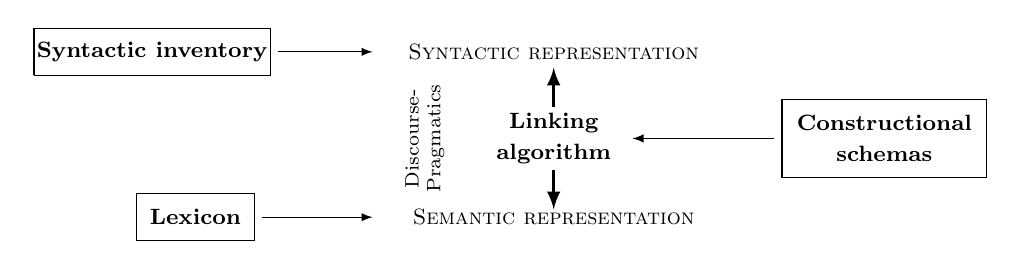
\begin{tikzpicture}
%%
\draw [xshift=0.75cm,yshift=1.3cm] node [] {{\bfseries\footnotesize{Lexicon}}};
\draw (0,1.0) -- (1.5,1.0) -- (1.5,1.6) -- (0,1.6) -- (0,1.0);
\draw [-latex] (1.6,1.3) -- (3,1.3) ;
\draw [xshift=5.3cm,yshift=1.3cm] node [] {{\scshape\footnotesize{Semantic representation}}};
%%
\draw [xshift=0.2cm,yshift=3.4cm] node [] {{\bfseries\footnotesize{Syntactic inventory}}};
\draw (-1.3,3.1) -- (1.7,3.1) -- (1.7,3.7) -- (-1.3,3.7) -- (-1.3,3.1);
\draw [-latex] (1.8,3.4) -- (3,3.4) ;
\draw [xshift=5.3cm,yshift=3.4cm] node [] {{\scshape\footnotesize{Syntactic representation}}};
%%
\draw [xshift=5.3cm,yshift=2.5cm] node [] {{\bfseries\footnotesize{Linking}}};
\draw [xshift=5.3cm,yshift=2.1cm] node [] {{\bfseries\footnotesize{algorithm}}};
%%
\draw [very thick,-latex] (5.3,2.7) -- (5.3,3.2) ;
\draw [very thick,-latex] (5.3,1.9) -- (5.3,1.4) ;
%%
\draw [xshift=9.5cm,yshift=2.5cm] node [] {{\bfseries\footnotesize{Constructional}}};
\draw [xshift=9.5cm,yshift=2.1cm] node [] {{\bfseries\footnotesize{schemas}}};
\draw (8.2,1.8) -- (10.8,1.8) -- (10.8,2.8) -- (8.2,2.8) -- (8.2,1.8);
\draw [-latex] (8.1,2.3) -- (6.3,2.3) ;
%%
\draw [xshift=3.5cm,yshift=2.3cm] node [rotate=90] {{\scriptsize{Discourse-}}};
\draw [xshift=3.8cm,yshift=2.3cm] node [rotate=90] {{\scriptsize{Pragmatics}}};
%%
\end{tikzpicture}
}
\caption{The general grammar architecure in RRG}
\label{fig:rrg:balogh}
\end{figure}

As \citet[][185]{vanvalin:05} argues by characterizing a ``cognitive model of context'', discourse pragmatics affects all aspects of the grammatical system \citep[for an overview see][]{bentley:23,lvv:23}. An essential part of discourse pragmatics is captured by the \textit{Focus Structure Projection} and its effects on the bi-directional linking between syntax and semantics. This projection, and the way of looking at \isi{IS} in \isi{RRG}, is based on the theory of \citet{lambrecht:94}, where the main contribution of focusing is a \textit{pragmatic structuring} into the \isi{pragmatic assertion} and the \isi{pragmatic presupposition}. As \citet{balogh:21} proposes, the projection should also model the topic-comment structure of the sentence for a comprehensive account of \isi{information structure} and for an appropriate account of various phenomena where focus-structure and topic-structure interact (e.g., the linearization constraints of the focus-sensitive particle \textit{also}). Following this proposal, we refer to the projection as the \textit{Information Structure (IS-)Projection}.\footnote{The topic-comment structure plays no direct role in the analysis of our target phenomenon; therefore, in this paper, we simplify the IS-Projection and discuss only the \isi{focus} structure.} 

The basic building blocks of the IS-Projection are the \textit{information units} (IUs) \citep[IUs; see][]{lambrecht:94,vanvalin:05,bentley:23}, that have a dual nature, linking both to the syntactic structure and to the semantic representation: IUs are linked to minimal phrasal units in the constituent structure and to their respective contents within the semantic representation. \isi{RRG} distinguishes two syntactic domains, both including one or more IUs: the \textit{potential \isi{focus} domain} (PFD), where the \isi{focus} can fall in the sentence, and the \textit{actual \isi{focus} domain} (AFD), whose content is considered the ``\isi{focus}'' in interpretational terms.\footnote{Note that the term \textit{\isi{focus} domain} is understood here within the terminology of \isi{RRG}.}
The notion of PFD is cross-linguistically relevant, and has an important role in the grammar theory. While, in English, the PFD is always the entire clause, this is not generally the case in other languages. For example, in Italian, the PFD excludes any core-internal pre-nuclear elements \citep[][]{vvlp:97,bentley:08}, and in Hungarian, the structural topic position is clause-internal, but external to the PFD. Therefore, the notion of PFD is central to capturing the structural restrictions on the location of \isi{focus} in various languages. Furthermore, as argued by \citet{vanvalin:05} and \citet{shimojo:23}, the PFD plays a crucial role in the explanation of \isi{focus} structure in complex sentences, and in the analysis of extraction phenomena. For the purposes of this paper, however, the notion of PFD has no direct relevance, therefore we omit a more detailed discussion of it. 

The general grammatical model of \isi{RRG} and the representation of \isi{IS} as the IS-Projection is considerably different from traditional accounts based on syntactic F-marking. The essence is that \isi{focus} domains are sets of IUs, linked to syntactic domains  but not determined by (or read off from) the nodes of the constituent structure. Once defined, any combination of basic IUs can make up the AFD/\isi{focus}. This predicts that non-constituent \isi{focus} structures are not problematic, and the different \isi{focus} structures can be captured via a uniform process. Despite the advantages that the \isi{RRG} approach offers to our target phenomena, the formal implementation of the theoretical grounds asks for a further development. The core issue is the formal modeling of IUs in a way that links them to syntactic domains and pieces of semantic information without a traditional implementation of compositionality. Regarding the aim of a uniform analysis of the possible \isi{focus} structures, a central question is at which point in the derivation and how the IUs are determined. 

\section{Formalization of the IS-Projection }\label{sec:form.is:Balogh}

In \isi{RRG}, the composition of the constituent structure (i.e., the layered structure of the clause) in the syntactic representation is the combination of tree templates in the syntactic inventory. However, the way these templates combine is left undefined and informal. Keeping the core of the theoretical base of \isi{RRG}, the use of a formalism based on Tree-Adjoining Grammar \citep[\isi{TAG};][]{joshi:schabes:97,ar:00} is a straightforward choice in the formalization of the syntactic combination. The formal specification of \isi{RRG} syntax is defined in terms of \textit{Tree-Wrapping Grammar} \citep[\isi{TWG};][]{kallm:etal:13,kallm:16}, which is strongly based on \isi{TAG}. The semantic representations are formalized in terms of \isi{decompositional frames} \citep[][]{barsalou:92,lobner:14,lobner:17,petersen:15}, formally defined as base-labeled typed feature structures \citep{kallm:ossw:13}. The current development of the formalization of \isi{RRG} provides a specification of the syntax-semantics interface, but lacks a model of \isi{IS}. We propose the necessary extension of the IS-Projection, towards a uniform formal representation of the various \isi{focus} structures.

\subsection{Grammar formalism for RRG: Tree-Wrapping Grammar }\label{sec:twg:Balogh}

The tree templates of \isi{RRG} are defined as the elementary trees of the \isi{TWG}, and they are combined by the rewriting operations of standard \textit{substitution} (\figref{fig:twg.syn:Balogh}a), where a leaf node is replaced by another tree, and \textit{(sister) adjunction} (\figref{fig:twg.syn:Balogh}b), where an internal node is replaced by another tree. For the derivation of certain constructions (e.g., extraction phenomena, control constructions), an additional, more complex substitution operation is proposed: \textit{wrapping substitution} \citep[see][750]{kallm:ossw:23}, where a tree is split at a special dominance edge and wrapped around the target tree. Given that in our examples this latter operation does not occur, we do not introduce it any further. For the exact definitions of the operations used for syntactic composition in \isi{TWG}, see \citet{kallm:etal:13} and \citet{kallm:ossw:23}.

\begin{figure}[H]
{\small{
(a)\hspace*{5cm}(b) 
}} \\
\centering
\scalebox{0.7}{
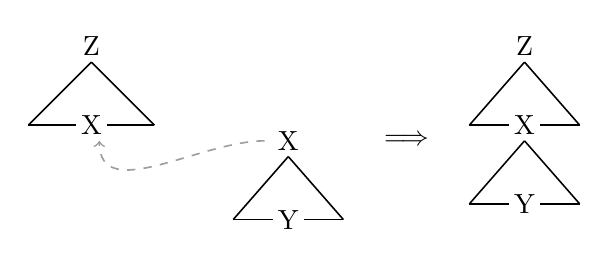
\begin{tikzpicture}[baseline]
\draw [xshift=1cm,yshift=2.2cm] node [] {Z}  ;
\draw [line width=0.2mm] (1.0,2.0) -- (0.2,1.2) ;
\draw [line width=0.2mm] (1.0,2.0) -- (1.8,1.2) ;
\draw [line width=0.2mm] (0.2,1.2) -- (0.8,1.2) ;
\draw [line width=0.2mm] (1.8,1.2) -- (1.2,1.2) ;
\draw [xshift=1cm,yshift=1.2cm] node [] {X}  ;
%%%%
\draw [xshift=3.5cm,yshift=1.0cm] node [] {X}  ;
\draw [line width=0.2mm] (3.5,0.8) -- (2.8,0.0) ;
\draw [line width=0.2mm] (3.5,0.8) -- (4.2,0.0) ;
\draw [line width=0.2mm] (2.8,0.0) -- (3.3,0.0) ;
\draw [line width=0.2mm] (4.2,0.0) -- (3.7,0.0) ;
\draw [xshift=3.5cm,yshift=0.0cm] node [] {Y}  ;
%%%
\draw[semithick,dashed,->,gray!75] (3.2,1.0) to [out=180, in=-90] (1.1,1.0);
%%%
\draw [xshift=5.0cm,yshift=1.0cm] node [] {$\Longrightarrow$}  ;
%%%
%%%%
\draw [xshift=6.5cm,yshift=2.2cm] node [] {Z}  ;
\draw [line width=0.2mm] (6.5,2.0) -- (5.8,1.2) ;
\draw [line width=0.2mm] (6.5,2.0) -- (7.2,1.2) ;
\draw [line width=0.2mm] (5.8,1.2) -- (6.3,1.2) ;
\draw [line width=0.2mm] (6.7,1.2) -- (7.2,1.2) ;
\draw [xshift=6.5cm,yshift=1.2cm] node [] {X}  ;
\draw [line width=0.2mm] (6.5,1.0) -- (5.8,0.2) ;
\draw [line width=0.2mm] (6.5,1.0) -- (7.2,0.2) ;
\draw [line width=0.2mm] (5.8,0.2) -- (6.3,0.2) ;
\draw [line width=0.2mm] (6.7,0.2) -- (7.2,0.2) ;
\draw [xshift=6.5cm,yshift=0.2cm] node [] {Y}  ;
\end{tikzpicture}
}
%%%%%%%%%%%
\hspace*{1cm}
%%%%%%%%%%%
\scalebox{0.7}{
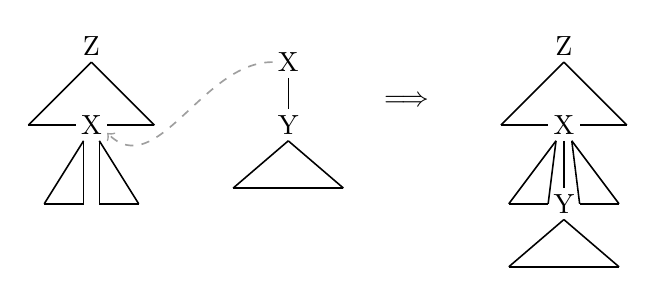
\begin{tikzpicture}[baseline]
\draw [xshift=1cm,yshift=2.2cm] node [] {Z}  ;
\draw [line width=0.2mm] (1.0,2.0) -- (0.2,1.2) ;
\draw [line width=0.2mm] (1.0,2.0) -- (1.8,1.2) ;
\draw [line width=0.2mm] (0.2,1.2) -- (0.8,1.2) ;
\draw [line width=0.2mm] (1.8,1.2) -- (1.2,1.2) ;
\draw [xshift=1cm,yshift=1.2cm] node [] {X}  ;
\draw [line width=0.2mm] (0.9,1.0) -- (0.9,0.2) ;
\draw [line width=0.2mm] (0.9,1.0) -- (0.4,0.2) ;
\draw [line width=0.2mm] (0.9,0.2) -- (0.4,0.2) ;
\draw [line width=0.2mm] (1.1,1.0) -- (1.1,0.2) ;
\draw [line width=0.2mm] (1.1,1.0) -- (1.6,0.2) ;
\draw [line width=0.2mm] (1.1,0.2) -- (1.6,0.2) ;
%%%
\draw [xshift=3.5cm,yshift=2.0cm] node [] {X}  ;
\draw [line width=0.2mm] (3.5,1.8) -- (3.5,1.4) ;
\draw [xshift=3.5cm,yshift=1.2cm] node [] {Y}  ;
\draw [line width=0.2mm] (3.5,1.0) -- (2.8,0.4) ;
\draw [line width=0.2mm] (3.5,1.0) -- (4.2,0.4) ;
\draw [line width=0.2mm] (2.8,0.4) -- (4.2,0.4) ;
%%%
\draw[semithick,dashed,->,gray!75] (3.3,2.0) to [out=180, in=-45] (1.2,1.1);
%%%
\draw [xshift=5.0cm,yshift=1.5cm] node [] {$\Longrightarrow$}  ;
%%%
\draw [xshift=7cm,yshift=2.2cm] node [] {Z}  ;
\draw [line width=0.2mm] (7.0,2.0) -- (6.2,1.2) ;
\draw [line width=0.2mm] (7.0,2.0) -- (7.8,1.2) ;
\draw [line width=0.2mm] (6.2,1.2) -- (6.8,1.2) ;
\draw [line width=0.2mm] (7.8,1.2) -- (7.2,1.2) ;
\draw [xshift=7cm,yshift=1.2cm] node [] {X}  ;
\draw [line width=0.2mm] (6.9,1.0) -- (6.8,0.2) ;
\draw [line width=0.2mm] (6.9,1.0) -- (6.3,0.2) ;
\draw [line width=0.2mm] (6.8,0.2) -- (6.3,0.2) ;
\draw [line width=0.2mm] (7.1,1.0) -- (7.2,0.2) ;
\draw [line width=0.2mm] (7.1,1.0) -- (7.7,0.2) ;
\draw [line width=0.2mm] (7.2,0.2) -- (7.7,0.2) ;
\draw [line width=0.2mm] (7.0,1.0) -- (7.0,0.4) ;
\draw [xshift=7.0cm,yshift=0.2cm] node [] {Y}  ;
\draw [line width=0.2mm] (7.0,0.0) -- (6.3,-0.6) ;
\draw [line width=0.2mm] (7.0,0.0) -- (7.7,-0.6) ;
\draw [line width=0.2mm] (6.3,-0.6) -- (7.7,-0.6) ;

\end{tikzpicture}
}

\caption{Substitution (a) and sister adjunction (b) in TWG} \label{fig:twg.syn:Balogh}
\end{figure}

One of the important characteristics of formalized \isi{RRG} representations is that the nodes in the tree representation are decorated with feature structures, including \textit{index features} ($I$) which establish the link between syntactic structure and semantic representation, hereby capturing essential aspects of the syntax-semantics interface (see \figref{ex:frrg.repr:Balogh}). Within \isi{RRG}, two oppositions are made prominent in the syntactic structure: (i) operators are distinguished from the predicate and its argument, and (ii) arguments are distinguished from adjunct \isi{modifiers}, where the latter are represented as ``periphery'' elements. In \isi{TWG}, we represent these distinctions as follows. The ``operator nodes'' are marked by OP-, together with the information of the operator type (OP-NEG for negation, OP-TNS for tense, OP-ASP for aspect, OP-DEF for definiteness, and so on). The information that an element is an adjunct \isi{modifier} is encoded in the {\textsc{peri+}} feature on the respective node. The {\textsc{pred+}} feature marks the respective node as predicative. 

\begin{figure}[H]
\scalebox{0.75}{
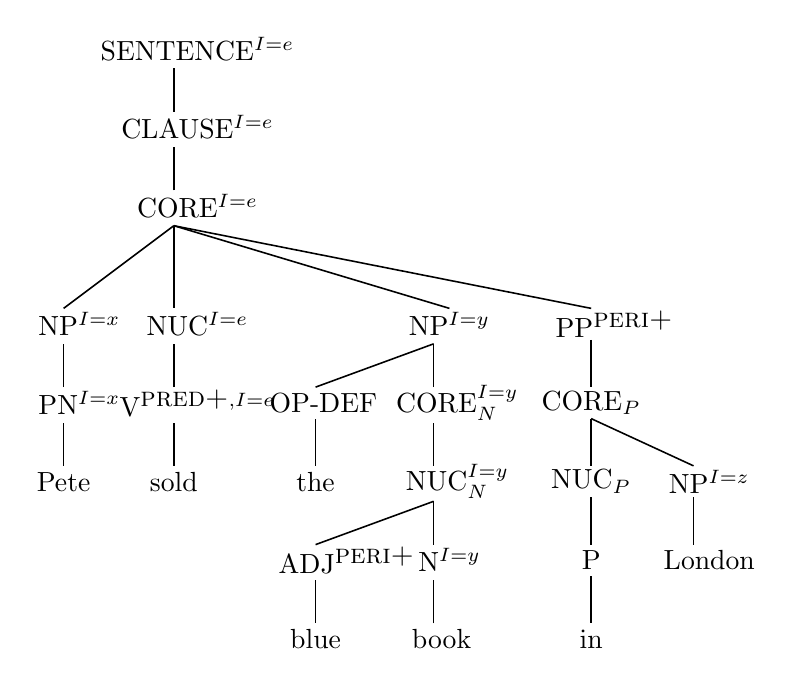
\begin{tikzpicture}[baseline=3cm]
\draw [xshift=1.5cm,yshift=5.5cm] node [] {SENTENCE$^{I=e}$};
\draw [line width=0.2mm] (1.2,4.7) -- (1.2,5.25) ;
\draw [xshift=1.5cm,yshift=4.5cm] node [] {CLAUSE$^{I=e}$};
\draw [line width=0.2mm] (1.2,3.7) -- (1.2,4.25) ;
\draw [xshift=1.5cm,yshift=3.5cm] node [] {CORE$^{I=e}$};
\draw [line width=0.2mm] (1.2,3.25) -- (-0.2,2.2) ;
\draw [line width=0.2mm] (1.2,3.25) -- (1.2,2.2) ;
\draw [line width=0.2mm] (1.2,3.25) -- (4.7,2.2) ;
\draw [line width=0.2mm] (1.2,3.25) -- (6.5,2.2) ;
%
\draw [xshift=1.5cm,yshift=2.0cm] node [] {NUC$^{I=e}$};
\draw [line width=0.2mm] (1.2,1.2) -- (1.2,1.75) ;
\draw [xshift=1.5cm,yshift=1.0cm] node [] {V$^{\text{\textsc{pred+}},I=e}$};
\draw [line width=0.2mm] (1.2,0.2) -- (1.2,0.75) ;
\draw [xshift=1.2cm,yshift=0.0cm] node [] {sold};
\draw [xshift=0.0cm,yshift=2.0cm] node [] {NP$^{I=x}$};
\draw [line width=0.2mm] (-0.2,1.2) -- (-0.2,1.75) ;
\draw [xshift=0.0cm,yshift=1.0cm] node [] {PN$^{I=x}$};
\draw [line width=0.2mm] (-0.2,0.2) -- (-0.2,0.75) ;
\draw [xshift=-0.2cm,yshift=0.0cm] node [] {Pete};
%%%%%%%% 
\draw [xshift=4.7cm,yshift=2.0cm] node [] {NP$^{I=y}$};
\draw [line width=0.2mm] (4.5,1.2) -- (4.5,1.75) ;
\draw [line width=0.2mm] (3.0,1.2) -- (4.5,1.75) ;
\draw [xshift=4.8cm,yshift=1.0cm] node [] {CORE$_{\text{N}}^{I=y}$};
\draw [line width=0.2mm] (4.5,0.2) -- (4.5,0.75) ;
\draw [xshift=4.8cm,yshift=0.0cm] node [] {NUC$_{\text{N}}^{I=y}$};
\draw [line width=0.2mm] (4.5,-0.8) -- (4.5,-0.25) ;
\draw [line width=0.2mm] (3.0,-0.8) -- (4.5,-0.25) ;
\draw [xshift=4.7cm,yshift=-1.0cm] node [] {N$^{I=y}$};
\draw [line width=0.2mm] (4.5,-1.8) -- (4.5,-1.25) ;
\draw [xshift=4.6cm,yshift=-2.0cm] node [] {book};
%%
\draw [xshift=3.1cm,yshift=1.0cm] node [] {OP-DEF};
\draw [line width=0.2mm] (3.0,0.2) -- (3.0,0.8) ;
\draw [xshift=3.0cm,yshift=0.0cm] node [] {the};
%%
\draw [xshift=3.4cm,yshift=-1.0cm] node [] {ADJ$^{\text{\textsc{peri+}}}$};
\draw [line width=0.2mm] (3.0,-1.25) -- (3.0,-1.8) ;
\draw [xshift=3.0cm,yshift=-2.0cm] node [] {blue};
%%%%%%%%% 
\draw [xshift=6.8cm,yshift=2.0cm] node [] {PP$^{\text{\textsc{peri+}}}$};
\draw [line width=0.2mm] (6.5,1.8) -- (6.5,1.2) ;
\draw [xshift=6.5cm,yshift=1.0cm] node [] {CORE$_{\text{P}}$};
\draw [line width=0.2mm] (6.5,0.8) -- (6.5,0.2) ;
\draw [line width=0.2mm] (6.5,0.8) -- (7.8,0.2) ;
\draw [xshift=6.5cm,yshift=0.0cm] node [] {NUC$_{\text{P}}$};
\draw [line width=0.2mm] (6.5,-0.2) -- (6.5,-0.8) ;
\draw [xshift=6.5cm,yshift=-1.0cm] node [] {P};
\draw [line width=0.2mm] (6.5,-1.2) -- (6.5,-1.8) ;
\draw [xshift=6.5cm,yshift=-2.0cm] node [] {in};
%%%
\draw [xshift=8.0cm,yshift=0.0cm] node [] {NP$^{I=z}$};
\draw [line width=0.2mm] (7.8,-0.8) -- (7.8,-0.2) ;
\draw [xshift=8.0cm,yshift=-1.0cm] node [] {London};
\end{tikzpicture}
}
%%%%%%%%%%%%%
\scalebox{0.8}{
\avm{
$e$[\type*{selling}
	actor 	& $x$[\type*{person} name & pete ]\\
	undergoer 	& $y$[\type*{book} color & blue ]\\
	location  & $z$[\type*{settlement} name & london ]\\	
]
}
}

\caption{Syntactic and semantic representation in formalized RRG}\label{ex:frrg.repr:Balogh}
\end{figure}

An important advantage of the formalization of \isi{RRG} with respect to the core theory of \isi{RRG} is that syntactic and semantic composition can be carried out on a par. A detailed discussion of the formalized theory goes beyond the scope of this paper, therefore we only provide a basic introduction here. Syntactic templates, i.e., elementary trees, are paired with pieces of semantic representations. We call these pairs \textit{elementary constructions}. The semantic composition is parallel to the syntactic composition, mediated by the index feature ($I$) on the nodes (\figref{fig:elem.frrg:Balogh}). The syntactic operations \citep[][]{kallm:etal:13} trigger the unification of the semantic representations, thereby deriving the meaning representation of the sentence. 

As shown in \figref{fig:elem.frrg:Balogh} below, the tree for the predicate is substituted at the NUC node, triggering $\boxed{0}=e$ and providing the type of the eventuality. The NP trees are substituted at the respective NP nodes, triggering $\boxed{1}=x$ and $\boxed{2}=y$. The tree for the definite article is adjoined at the NP node of tree for \textit{book}, triggering $\boxed{3}=y$,  and the tree for the adjective \textit{red} is adjoined at its NUC$_{\text{N}}$ node, triggering $\boxed{4}=y$. The tree for the preposition \textit{in} is (sister) adjoined at the CORE node of the tree for the predicate, triggering $\boxed{5}=e$, and the tree for \textit{London} is substituted at the NP node within the tree for \textit{in}, triggering $\boxed{6}=z$. In the derived semantic representation, the pieces of the meaning representations within the elementary constructions are unified under these restrictions. The derived construction, the  syntactic tree and the corresponding semantic representation as a frame structure, is the one given in \figref{ex:frrg.repr:Balogh} above.

\begin{figure}[H]
\scalebox{0.75}{
\begin{tikzpicture}[baseline=3cm]
\draw [xshift=2.0cm,yshift=5.1cm] node [] {SENTENCE$^{I=\boxed{0}}$};
\draw [line width=0.2mm] (1.8,4.75) -- (1.8,4.2) ;
\draw [xshift=2.0cm,yshift=4.1cm] node [] {CLAUSE$^{I=\boxed{0}}$};
\draw [line width=0.2mm] (1.8,3.8) -- (1.8,3.2) ;
\draw [xshift=2.0cm,yshift=3.1cm] node [] {CORE$^{I=\boxed{0}}$};
\draw [line width=0.2mm] (1.8,2.8) -- (0.2,2.2) ;
\draw [line width=0.2mm] (1.8,2.8) -- (1.8,2.2) ;
\draw [line width=0.2mm] (1.8,2.8) -- (3.2,2.2) ;
\draw [xshift=2.0cm,yshift=2.1cm] node [] {NUC$^{I=\boxed{0}}$};
%
\draw [xshift=0.5cm,yshift=2.0cm] node [] {NP$^{I=\boxed{1}}$};
\draw [xshift=3.6cm,yshift=2.0cm] node [] {NP$^{I=\boxed{2}}$};
%
\draw [xshift=-0.8cm,yshift=4.0cm] node [] { 
\avm{
$\boxed{0}$[\type*{event}
	actor 	& $\boxed{1}$ \\
	undg	& $\boxed{2}$ 
]
}
} ; 
%%%%
\draw[semithick,dashed,->,gray!75] (1.3,1.0) to [out=180, in=-90] (1.6,1.7) ;
\draw [xshift=2.0cm,yshift=1.0cm] node [] {NUC$^{I=e}$};
\draw [line width=0.2mm] (1.8,0.75) -- (1.8,0.2) ;
\draw [xshift=2.45cm,yshift=0.0cm] node [] {V$^{{\textsc{pred+}},I=e}$};
\draw [line width=0.2mm] (1.8,-0.25) -- (1.8,-0.8) ;
\draw [xshift=1.8cm,yshift=-1.0cm] node [] {sold};
%
\draw [xshift=2.0cm,yshift=-2.2cm] node [] { 
\avm{
$e$[\type*{selling}
	actor 	& $q$ \\
	undg	& $r$ 
]
}
} ; 
%%%%%%%%%%%%%%%%%%%%%%%%%
\draw [xshift=-0.8cm,yshift=1.0cm] node [] {NP$^{I=x}$};
\draw [line width=0.2mm] (-1.0,0.8) -- (-1.0,0.2) ;
\draw [xshift=-1.0cm,yshift=0.0cm] node [] {Pete};
%%
\draw [xshift=-1.0cm,yshift=-0.8cm] node [] { 
\avm{
$x$[\type*{person} name & pete ]
}
} ; 
\draw[semithick,dashed,->,gray!75] (-1.0,1.15) to [out=90, in=-90] (0.1,1.70) ;
%%%%%%%%%%%%%%%%%%%%%%%%%
\draw [xshift=4.3cm,yshift=0.0cm] node [] {NP$^{I=\boxed{3}}$};
\draw [line width=0.2mm] (4.0,-0.3) -- (4.0,-0.8) ;
\draw [xshift=4.0cm,yshift=-1.0cm] node [] {OP-DEF};
\draw [line width=0.2mm] (4.0,-1.2) -- (4.0,-1.8) ;
\draw [xshift=4.0cm,yshift=-2.0cm] node [] {the};
%%
\draw [xshift=4.0cm,yshift=-2.7cm] node [] { 
\avm{
$\boxed{3}$[ ]
}
} ; 
\draw[semithick,dashed,->,gray!75] (4.95,-0.1) to [out=0, in=180] (7.15,1.0) ;
%%%%%%%%%%%%%%%%%%%%%%%%%
\draw [xshift=5.8cm,yshift=-1.5cm] node [] {NUC$_{\text{N}}^{I=\boxed{4}}$};
\draw [line width=0.2mm] (5.5,-1.8) -- (5.5,-2.3) ;
\draw [xshift=5.8cm,yshift=-2.5cm] node [] {AP$^{{\textsc{peri+}}}$};
\draw [line width=0.2mm] (5.5,-2.7) -- (5.5,-3.3) ;
\draw [xshift=5.5cm,yshift=-3.5cm] node [] {blue};
%%
\draw [xshift=5.3cm,yshift=-4.2cm] node [] { 
\avm{
$\boxed{4}$[ color & blue ]
}
} ; 
\draw[semithick,dashed,->,gray!75] (5.5,-1.3) to [out=90, in=180] (7.0,-1.0) ;
%%%%%%%%%%%%%%%%%%%%%%%%%
\draw [xshift=7.7cm,yshift=1.0cm] node [] {NP$^{I=y}$};
\draw [line width=0.2mm] (7.5,0.78) -- (7.5,0.2) ;
\draw [xshift=7.7cm,yshift=0.0cm] node [] {CORE$_{\text{N}}^{I=y}$};
\draw [line width=0.2mm] (7.5,-0.25) -- (7.5,-0.8) ;
\draw [xshift=7.7cm,yshift=-1.0cm] node [] {NUC$_{\text{N}}^{I=y}$};
\draw [line width=0.2mm] (7.5,-1.25) -- (7.5,-1.8) ;
\draw [xshift=7.7cm,yshift=-2.0cm] node [] {N$^{I=y}$};
\draw [line width=0.2mm] (7.5,-2.25) -- (7.5,-2.8) ;
\draw [xshift=7.5cm,yshift=-3.0cm] node [] {book};
%%
\draw [xshift=7.5cm,yshift=-3.7cm] node [] { 
\avm{
$y$[\type*{book} ]
}
} ; 
\draw[semithick,dashed,->,gray!75] (7.4,1.2) to [out=90, in=-90] (3.3,1.7) ;
%%%%%%%%%%%%%%%%%%%%%%%%%
\draw [xshift=9.7cm,yshift=3.0cm] node [] {CORE$^{I=\boxed{5}}$};
\draw [line width=0.2mm] (9.4,2.7) -- (9.4,2.2) ;
\draw [xshift=9.7cm,yshift=2.0cm] node [] {PP$^{I=\boxed{5}}$};
\draw [line width=0.2mm] (9.4,1.8) -- (9.4,1.2) ;
\draw [xshift=9.6cm,yshift=1.0cm] node [] {CORE$_{\text{P}}^{I=\boxed{5}}$};
\draw [line width=0.2mm] (9.4,0.2) -- (9.4,0.8) ;
\draw [xshift=9.6cm,yshift=0.0cm] node [] {NUC$_{\text{P}}^{I=\boxed{5}}$};
\draw [line width=0.2mm] (9.4,-0.25) -- (9.4,-0.85) ;
\draw [line width=0.2mm] (9.4,-0.25) -- (10.5,-0.85) ;
\draw [xshift=9.7cm,yshift=-1.0cm] node [] {P$^{I=\boxed{5}}$};
\draw [line width=0.2mm] (9.4,-1.3) -- (9.4,-1.8) ;
\draw [xshift=9.4cm,yshift=-2.0cm] node [] {in};
\draw [xshift=10.9cm,yshift=-1.0cm] node [] {NP$^{I=\boxed{6}}$};
%%
\draw [xshift=9.5cm,yshift=-2.5cm] node [] { 
\avm{
$\boxed{5}$[ loc & $\boxed{6}$ ]
}
} ; 
\draw[semithick,dashed,->,gray!75] (9.4,3.2) to [out=130, in=0] (2.9,2.9) ;
%%%%%%%%%%%%%%%%%%%%%%%%%
\draw [xshift=11.5cm,yshift=-2.0cm] node [] {NP$^{I=z}$};
\draw [line width=0.2mm] (11.5,-2.2) -- (11.5,-2.8) ;
\draw [xshift=11.5cm,yshift=-3.0cm] node [] {London};
%%
\draw [xshift=11.5cm,yshift=-3.9cm] node [] { 
\avm{
$z$[\type*{settlement} name & london ]
}
} ; 
\draw[semithick,dashed,->,gray!75] (11.2,-1.8) to [out=90, in=-90] (10.5,-1.3) ;
%%%%%%%%%%%%%%%%%%%%%%%%%
\end{tikzpicture}
}

\caption{Elementary constructions and their composition}\label{fig:elem.frrg:Balogh}
\end{figure}


\subsection{Formal representation of the information units}\label{sec:form.ius:Balogh}

While the syntactic and semantic operations are fairly worked out in formalized \isi{RRG}, the formalization of \isi{RRG}'s IS-Projection, an important mediator between syntax and semantics in the grammar architecture, is still missing.

In the theory of \isi{RRG} \citep{vanvalin:05}, \isi{IS} is represented in a separate module, which is linked both to syntax and semantics. The basic components of the IS-Projection are the {\emph{information units}} (IUs). They correspond to single syntactic constituents \citep[][]{vanvalin:05,bentley:23} and their respective content. Following \citet{lambrecht:94}, the basic IUs correspond to the content of the minimal phrasal categories in the constituent structure \citep[][78]{vanvalin:05}, i.e., the  sub-trees corresponding to the NUCLEUS, the core arguments (NP and PPs) and the periphery adjuncts (PPs), as indicated by the dashed box in \figref{ex:basic.ius.syn:Balogh}. Hence, IUs are linked both to syntactic domains (sub-trees) and their respective semantic representations. 

\begin{figure}[H]
\centering
\begin{minipage}{7cm}
\scalebox{0.8}{
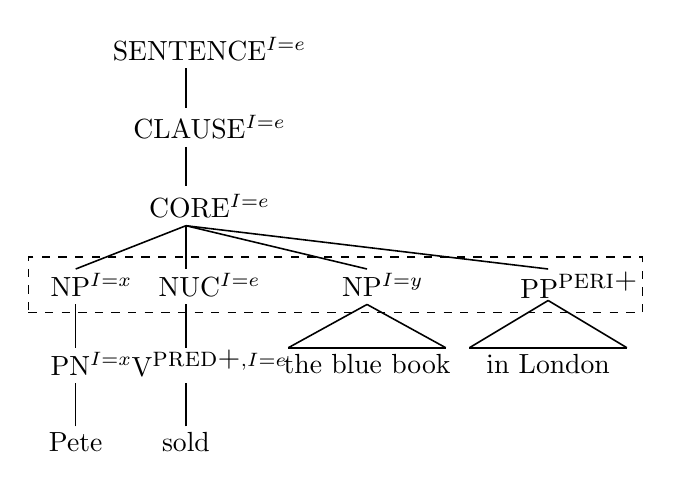
\begin{tikzpicture}[baseline=3cm]
\draw [xshift=1.5cm,yshift=5.0cm] node [] {SENTENCE$^{I=e}$};
\draw [line width=0.2mm] (1.2,4.75) -- (1.2,4.25) ;
\draw [xshift=1.5cm,yshift=4.0cm] node [] {CLAUSE$^{I=e}$};
\draw [line width=0.2mm] (1.2,3.75) -- (1.2,3.25) ;
\draw [xshift=1.5cm,yshift=3.0cm] node [] {CORE$^{I=e}$};
\draw [line width=0.2mm] (1.2,2.75) -- (-0.2,2.2) ;
\draw [line width=0.2mm] (1.2,2.75) -- (1.2,2.2) ;
\draw [line width=0.2mm] (1.2,2.75) -- (3.5,2.2) ;
\draw [line width=0.2mm] (1.2,2.75) -- (5.8,2.2) ;
%%%%%%%%
\draw [xshift=1.5cm,yshift=2.0cm] node [] {NUC$^{I=e}$};
\draw [line width=0.2mm] (1.2,1.2) -- (1.2,1.75) ;
\draw [xshift=1.5cm,yshift=1.0cm] node [] {V$^{\text{\textsc{pred+}},I=e}$};
\draw [line width=0.2mm] (1.2,0.2) -- (1.2,0.75) ;
\draw [xshift=1.2cm,yshift=0.0cm] node [] {sold};
%%%%%%%%
\draw [xshift=0.0cm,yshift=2.0cm] node [] {NP$^{I=x}$};
\draw [line width=0.2mm] (-0.2,1.2) -- (-0.2,1.75) ;
\draw [xshift=0.0cm,yshift=1.0cm] node [] {PN$^{I=x}$};
\draw [line width=0.2mm] (-0.2,0.2) -- (-0.2,0.75) ;
\draw [xshift=-0.2cm,yshift=0.0cm] node [] {Pete};
%%%%%%%%
\draw [xshift=3.7cm,yshift=2.0cm] node [] {NP$^{I=y}$};
\draw [line width=0.2mm] (3.5,1.75) -- (2.5,1.2) ;
\draw [line width=0.2mm] (3.5,1.75) -- (4.5,1.2) ;
\draw [line width=0.2mm] (2.5,1.2) -- (4.5,1.2) ;
\draw [xshift=3.5cm,yshift=1.0cm] node [] {the blue book};
%%%%%%%%%%
\draw [xshift=6.2cm,yshift=2.0cm] node [] {PP$^{\text{\textsc{peri+}}}$};
\draw [line width=0.2mm] (5.8,1.8) -- (4.8,1.2) ;
\draw [line width=0.2mm] (5.8,1.8) -- (6.8,1.2) ;
\draw [line width=0.2mm] (4.8,1.2) -- (6.8,1.2) ;
\draw [xshift=5.8cm,yshift=1.0cm] node [] {in London};
%%%%%%%%%% 
\draw [line width=0.2mm,dashed ] (-0.8,1.65) -- (7.0,1.65) -- (7.0,2.35) -- (-0.8,2.35) -- (-0.8,1.65) ;
\end{tikzpicture}
}
\end{minipage}
%%%%%%%%%%%%%%%%
\begin{minipage}{5cm}
\isi{IU} linked to the first NP: \\[2mm]
\scalebox{0.85}{
	\avm{
	$x$[\type*{person} name & pete ] 
	}
	} \\[3mm]
\isi{IU} linked to the second NP: \\[2mm]
\scalebox{0.85}{
	\avm{
	$y$[\type*{book} color & blue ] 
	}
	} \\
\end{minipage}

\caption{The syntactic domains of basic IUs}\label{ex:basic.ius.syn:Balogh}
\end{figure}

The IUs linked to the argument NPs are such that their content can be directly determined on the final semantic representation (see \figref{ex:frrg.repr:Balogh}) by pointing at the corresponding nodes labeled $x$ and $y$ in the frame. The IUs corresponding to the NUCLEUS and the adjunct PP are different, as their content cannot be addressed via frame nodes. Each clause has a unique NUCLEUS, that expresses the type of the eventuality (\ref{ex:iu-nucleus:Balogh}). The  content of the periphery PP in the case at stake includes that the location of some unspecified eventuality is London (\ref{ex:iu-pp:Balogh}). 

\ea
    \ea \isi{IU} corresponding to the NUCLEUS: \label{ex:iu-nucleus:Balogh}\\[1mm]
	\scalebox{0.85}{
	\avm{
	$e$[\type*{selling} actor & $q$ \\ undergoer & $r$ ] 
	}}
    \ex \isi{IU} corresponding to the PP$^{\textsc{peri+}}$: \label{ex:iu-pp:Balogh}\\[1mm]
    \scalebox{0.85}{
	\avm{
	$\boxed{5}$[ location & $z$ [\type*{settlement} name & london ] ] 
	}}
    \z
\z

The IUs correspond to the content of certain syntactic domains, i.e., sub-trees in the constituent structure. Despite the clear intuitions regarding what semantic contents are contributed by these sub-trees, the question arises of how to reach or how to derive all basic IUs in a uniform way, in other words, how they are determined in the formal model. We propose that the content of the syntactic domains linked to the basic IUs are determined by the ``derivation tree'', adapted from the \isi{TAG} formalisms. 

In a \isi{TAG} derivation, in addition to the final phrase structure tree (called the ``derived tree''), a ``derivation tree'' is given, which uniquely describes the \isi{TAG} derivation in question, i.e., which trees are combined at which nodes. The derivation tree contains nodes for all elementary trees used in the derivation, edges for all syntactic compositions performed throughout the derivation, and edge labels indicating the target node of the given syntactic operation. For referring to the nodes in the elementary trees, Gorn addresses \citep{gorn:67} are used, where the root node of the tree has address 0, and the $i^{th}$ daughter of the node with address $n$ has address $ni$. Whenever an elementary tree $\gamma$ rewrites the node at Gorn address $n$ in the elementary tree $\gamma'$, there is an edge from  $\gamma'$ to $\gamma$ labeled with $n$ (see \ref{ex:deriv.tree:Balogh}a).

\ea\label{ex:deriv.tree:Balogh}
a. Gorn addresses: \hspace*{2cm}b. Derivation tree for \figref{fig:elem.frrg:Balogh}:\\
\begin{minipage}{5cm}
{\scalebox{0.8}{
\begin{forest} 
[0
    [1 [11 ] [12 [121 ] ] [13 ] ]
    [2 [21 [211 ] [212 ] ] [22 [221 ] ] ]
]
\end{forest}
}}
\vspace*{10mm}
\end{minipage}
%%%
\begin{minipage}{6.2cm}
\scalebox{0.85}{
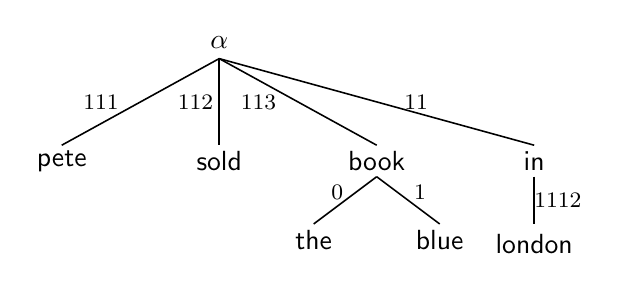
\begin{tikzpicture}[baseline=1cm]
\draw [xshift=2.0cm,yshift=1.5cm] node [] {$\alpha$}  ;
\draw [line width=0.2mm] (2.0,1.3) -- (0,0.2) ;
\draw [xshift=0.5cm,yshift=0.75cm] node [] {\footnotesize{111}}  ;
\draw [xshift=0.0cm,yshift=0cm] node [] {\sffamily{pete}} ;

\draw [line width=0.2mm] (2.0,1.3) -- (2.0,0.2) ;
\draw [xshift=1.7cm,yshift=0.75cm] node [] {\footnotesize{112}}  ;
\draw [xshift=2.0cm,yshift=0cm] node [] {\sffamily{sold}} ;

\draw [line width=0.2mm] (2.0,1.3) -- (4.0,0.2) ;
\draw [xshift=2.5cm,yshift=0.75cm] node [] {\footnotesize{113}}  ;
\draw [xshift=4.0cm,yshift=0cm] node [] {\sffamily{book}} ;

\draw [line width=0.2mm] (4.0,-0.2) -- (3.2,-0.8) ;
\draw [xshift=3.5cm,yshift=-0.4cm] node [] {\footnotesize{0}}  ;
\draw [xshift=3.2cm,yshift=-1.0cm] node [] {\sffamily{the}} ;

\draw [line width=0.2mm] (4.0,-0.2) -- (4.8,-0.8) ;
\draw [xshift=4.55cm,yshift=-0.4cm] node [] {\footnotesize{1}}  ;
\draw [xshift=4.8cm,yshift=-1.0cm] node [] {\sffamily{blue}} ;

\draw [line width=0.2mm] (2.0,1.3) -- (6.0,0.2) ;
\draw [xshift=4.5cm,yshift=0.75cm] node [] {\footnotesize{11}}  ;
\draw [xshift=6.0cm,yshift=0cm] node [] {\sffamily{in}} ;

\draw [line width=0.2mm] (6.0,-0.2) -- (6.0,-0.8) ;
\draw [xshift=6.3cm,yshift=-0.5cm] node [] {\footnotesize{1112}}  ;
\draw [xshift=6.0cm,yshift=-1.05cm] node [] {\sffamily{london}} ;
%
\end{tikzpicture}
}%
\\
inducing the unification of the frames under: 
$\boxed{1}=e$, $\boxed{1}=x$,\\[1mm] $\boxed{2}=\boxed{3}=\boxed{4}=y$, $\boxed{5}=e$, $\boxed{6}=z$
\end{minipage}
\z

In the derivation of the sentence \textit{Pete sold the blue book in London} (see \ref{ex:deriv.tree:Balogh}b), the tree for the base structure of a transitive construction (referred to by $\alpha$ here) has three substitution nodes, one labeled NUC and two labeled NP. The tree for \textit{Pete} is substituted at node 111, the tree for \textit{sold} at node 112  and the tree for \textit{book} at node 113. The tree for \textit{in} is adjoined (by sister adjunction) to $\alpha$ at node 11. The trees for \textit{the} and \textit{blue} are (sister) adjoined to the tree for \textit{book} at nodes 0 (root) and 1 respectively, and finally, the tree for \textit{London} is substituted at node 1112 to the tree for \textit{in}. All these operations are registered in the derivation tree (\ref{ex:deriv.tree:Balogh}b), which implicitly includes the respective unifications of the corresponding pieces of semantic content. For example, the node labeled `{\sffamily{book}}' stands for the elementary construction of the pair of the elementary tree anchored by the noun {\emph{book}} and its corresponding semantic frame. 
 
We propose that the information units, i.e., the designated syntactic domains and their content, correspond to the non-operator daughter sub-trees of the root node of the derivation tree. Together with the information on the substitution/adjunction sites of each of these parts -- what is also described by the derivation tree -- we derive the set of \isi{IU} contents in the given sentence (\figref{fig:deriv.tree.ius:Balogh}). We refer to this set as IUS.

\begin{figure}[H]

\scalebox{0.9}{
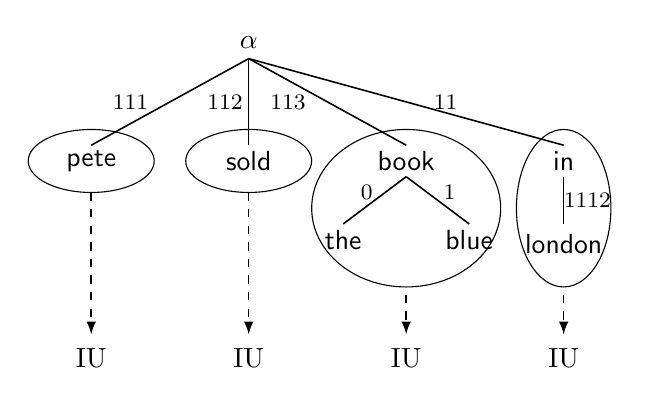
\begin{tikzpicture}[baseline=1cm]
\draw [xshift=2.0cm,yshift=1.5cm] node [] {$\alpha$}  ;
\draw [line width=0.2mm] (2.0,1.3) -- (0,0.2) ;
\draw [xshift=0.5cm,yshift=0.75cm] node [] {\footnotesize{111}}  ;
\draw [xshift=0.0cm,yshift=0cm] node [] {\sffamily{pete}} ;

\draw [line width=0.2mm] (2.0,1.3) -- (2.0,0.2) ;
\draw [xshift=1.7cm,yshift=0.75cm] node [] {\footnotesize{112}}  ;
\draw [xshift=2.0cm,yshift=0cm] node [] {\sffamily{sold}} ;

\draw [line width=0.2mm] (2.0,1.3) -- (4.0,0.2) ;
\draw [xshift=2.5cm,yshift=0.75cm] node [] {\footnotesize{113}}  ;
\draw [xshift=4.0cm,yshift=0cm] node [] {\sffamily{book}} ;

\draw [line width=0.2mm] (4.0,-0.2) -- (3.2,-0.8) ;
\draw [xshift=3.5cm,yshift=-0.4cm] node [] {\footnotesize{0}}  ;
\draw [xshift=3.2cm,yshift=-1.0cm] node [] {\sffamily{the}} ;

\draw [line width=0.2mm] (4.0,-0.2) -- (4.8,-0.8) ;
\draw [xshift=4.55cm,yshift=-0.4cm] node [] {\footnotesize{1}}  ;
\draw [xshift=4.8cm,yshift=-1.0cm] node [] {\sffamily{blue}} ;

\draw [line width=0.2mm] (2.0,1.3) -- (6.0,0.2) ;
\draw [xshift=4.5cm,yshift=0.75cm] node [] {\footnotesize{11}}  ;
\draw [xshift=6.0cm,yshift=0cm] node [] {\sffamily{in}} ;

\draw [line width=0.2mm] (6.0,-0.2) -- (6.0,-0.8) ;
\draw [xshift=6.3cm,yshift=-0.5cm] node [] {\footnotesize{1112}}  ;
\draw [xshift=6.0cm,yshift=-1.05cm] node [] {\sffamily{london}} ;
%
\draw (0.0,0.0) ellipse (0.8cm and 0.4cm);
\draw (2.0,0.0) ellipse (0.8cm and 0.4cm);
\draw (4.0,-0.6) ellipse (1.2cm and 1.0cm);
\draw (6.0,-0.6) ellipse (0.6cm and 1.0cm);
%%%
\draw [line width=0.2mm,dashed,-latex] (0.0,-0.4) -- (0.0,-2.2) ;
\draw [line width=0.2mm,dashed,-latex] (2.0,-0.4) -- (2.0,-2.2) ;
\draw [line width=0.2mm,dashed,-latex] (4.0,-1.7) -- (4.0,-2.2) ;
\draw [line width=0.2mm,dashed,-latex] (6.0,-1.7) -- (6.0,-2.2) ;
%%%
\draw [xshift=0.0cm,yshift=-2.5cm] node [] {IU} ;
\draw [xshift=2.0cm,yshift=-2.5cm] node [] {IU} ;
\draw [xshift=4.0cm,yshift=-2.5cm] node [] {IU} ;
\draw [xshift=6.0cm,yshift=-2.5cm] node [] {IU} ;
\end{tikzpicture}
}

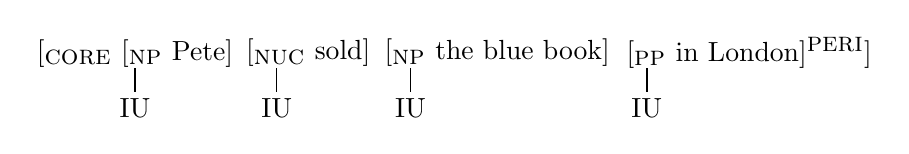
\begin{tikzpicture}[]
    \draw [xshift=0.0cm,yshift=0.99cm] node [] {[$_{\textsc{core}}$ [$_{\textsc{np}}$ Pete]}  ;
    \draw [xshift=2.2cm,yshift=1.0cm] node [] {[$_{\textsc{nuc}}$ sold]}  ;
    \draw [xshift=4.6cm,yshift=1.0cm] node [] {[$_{\textsc{np}}$ the blue book]}  ;
    \draw [xshift=7.8cm,yshift=1.0cm] node [] {[$_{\textsc{pp}}$ in London]$^{\textsc{peri}}$]}  ;
    %%
    \draw [line width=0.2mm] (0.0,0.8) -- (0.0,0.5) ;
    \draw [line width=0.2mm] (1.8,0.8) -- (1.8,0.5) ;
    \draw [line width=0.2mm] (3.5,0.8) -- (3.5,0.5) ;
    \draw [line width=0.2mm] (6.5,0.8) -- (6.5,0.5) ;
    %%
    \draw [xshift=0.0cm,yshift=0.3cm] node [] {IU}  ;
    \draw [xshift=1.8cm,yshift=0.3cm] node [] {IU}  ;
    \draw [xshift=3.5cm,yshift=0.3cm] node [] {IU}  ;
    \draw [xshift=6.5cm,yshift=0.3cm] node [] {IU}  ;
%%%%%%%%%%%%%%%%
\end{tikzpicture}

\scalebox{0.8}{
    \avm{$x$[\type*{person} name & pete ]} 
},
\scalebox{0.8}{
    \avm{$e$[\type*{selling} 
    actor & $\boxed{1}$\\
    undg & $\boxed{2}$]}
}, 
\scalebox{0.8}{
    \avm{$y$[\type*{book} color & blue ]}
},
\scalebox{0.8}{
    \avm{
    $\boxed{5}$[
    loc & $z$[\type*{settlement} name & london ]]}
}

\caption{Derivation tree and the set of information units }\label{fig:deriv.tree.ius:Balogh}
\end{figure}

The basic IUs are the minimal elements of the various IS-domains, such as the actual \isi{focus} domain, the comment and so on. These IS-domains are formally defined as subsets of the IUS. The minimal \isi{focus} domains correspond to basic IUs, but not vice versa: not every basic \isi{IU} can be part of a \isi{focus} domain. Therefore, we can model the potential \isi{focus} domain (PFD) as the set of all minimal \isi{focus} domains (MFDs). These minimal \isi{focus} domains can be marked by the feature \textsc{mfd+} on given nodes in the constituent tree, which is language-specific. 

%%%% CHECK THIS OUT!!!!!


\section{Focus structures }\label{sec:foc.structs:Balogh}

The basic idea of a uniform representation of different \isi{focus} structures is relatively simple: within the IS-Projection, the IS-domains are formally represented as sets of IUs. This provides the necessary flexibility to deal with non-constituent \isi{focus}, since \isi{focus} structure is not directly determined on the syntactic tree. Note that the relation to the syntactic structure is not lost, as determining the basic information units is based on syntactic domains. For the aims of this paper, two IS-domains are directly relevant: the {\textsc{focus}} (corresponding to \isi{RRG}'s AFD) and the {\textsc{non-focus}}. Both are subsets of the set IUS, structurally determined as shown before. The {\textsc{focus}} (F) is a non-empty subset of the IUS, and the {\textsc{non-focus}} (NF) is the (possibly empty) complement set of the {\textsc{focus}} with respect to the IUS. The partition to these IS-domains is the core of the representation of all \isi{focus} structures, as illustrated in (\ref{ex:obj-foc:Balogh}) for \isi{object} \isi{focus} structures or in (\ref{ex:subj-Vfoc:Balogh}) for subject-verb \isi{focus} structures. 

\ea Example \isi{focus} structures
    \ea \isi{object} \isi{focus}: \label{ex:obj-foc:Balogh}\\
    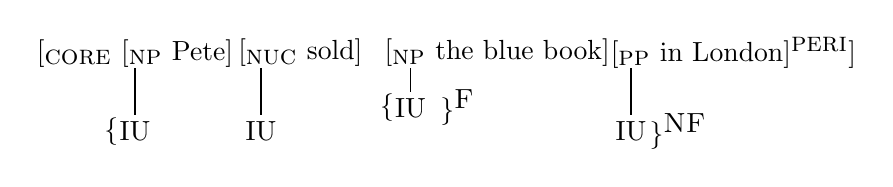
\begin{tikzpicture}[]
    \draw [xshift=0.0cm,yshift=0.99cm] node [] {[$_{\textsc{core}}$ [$_{\textsc{np}}$ Pete]}  ;
    \draw [xshift=2.1cm,yshift=1.0cm] node [] {[$_{\textsc{nuc}}$ sold]}  ;
    \draw [xshift=4.6cm,yshift=1.0cm] node [] {[$_{\textsc{np}}$ the blue book]}  ;
    \draw [xshift=7.6cm,yshift=1.0cm] node [] {[$_{\textsc{pp}}$ in London]$^{\textsc{peri}}$]}  ;
    %%
    \draw [line width=0.2mm] (0.0,0.8) -- (0.0,0.2) ;
    \draw [line width=0.2mm] (1.6,0.8) -- (1.6,0.2) ;
    \draw [line width=0.2mm] (3.5,0.8) -- (3.5,0.5) ;
    \draw [line width=0.2mm] (6.3,0.8) -- (6.3,0.2) ;
    %%
    \draw [xshift=0.0cm,yshift=0.0cm] node [] {IU}  ;
    \draw [xshift=1.6cm,yshift=0.0cm] node [] {IU}  ;
    \draw [xshift=3.5cm,yshift=0.3cm] node [] {IU}  ;
    \draw [xshift=6.3cm,yshift=0.0cm] node [] {IU}  ;
    %%
    \draw [xshift=-0.3cm,yshift=0.0cm] node [] {\{} ;
    \draw [xshift=6.9cm,yshift=0.0cm] node [] {\}$^{\textsc{NF}}$} ;
    \draw [xshift=3.2cm,yshift=0.3cm] node [] {\{} ;
    \draw [xshift=4.1cm,yshift=0.3cm] node [] {\}$^{\textsc{F}}$} ;
    \end{tikzpicture}    
%%%%%%%%%%%%%%%%%%%%%%%%%%%%%%%%%%%%%%%%%%%%%%%%%%%%%%%
    \ex \isi{subject} + V \isi{focus}: \label{ex:subj-Vfoc:Balogh}\\
    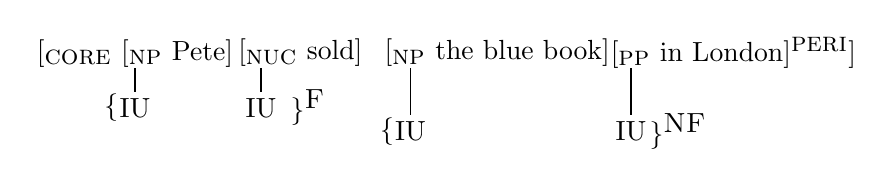
\begin{tikzpicture}[]
    \draw [xshift=0.0cm,yshift=0.99cm] node [] {[$_{\textsc{core}}$ [$_{\textsc{np}}$ Pete]}  ;
    \draw [xshift=2.1cm,yshift=1.0cm] node [] {[$_{\textsc{nuc}}$ sold]}  ;
    \draw [xshift=4.6cm,yshift=1.0cm] node [] {[$_{\textsc{np}}$ the blue book]}  ;
    \draw [xshift=7.6cm,yshift=1.0cm] node [] {[$_{\textsc{pp}}$ in London]$^{\textsc{peri}}$]}  ;
    %%
    \draw [line width=0.2mm] (0.0,0.8) -- (0.0,0.5) ;
    \draw [line width=0.2mm] (1.6,0.8) -- (1.6,0.5) ;
    \draw [line width=0.2mm] (3.5,0.8) -- (3.5,0.2) ;
    \draw [line width=0.2mm] (6.3,0.8) -- (6.3,0.2) ;
    %%
    \draw [xshift=0.0cm,yshift=0.3cm] node [] {IU}  ;
    \draw [xshift=1.6cm,yshift=0.3cm] node [] {IU}  ;
    \draw [xshift=3.5cm,yshift=0.0cm] node [] {IU}  ;
    \draw [xshift=6.3cm,yshift=0.0cm] node [] {IU}  ;
    %%
    \draw [xshift=3.2cm,yshift=0.0cm] node [] {\{} ;
    \draw [xshift=6.9cm,yshift=0.0cm] node [] {\}$^{\textsc{NF}}$} ;
    \draw [xshift=-0.3cm,yshift=0.3cm] node [] {\{} ;
    \draw [xshift=2.2cm,yshift=0.3cm] node [] {\}$^{\textsc{F}}$} ;
    \end{tikzpicture}
    \z
\z

How to derive these partitions is a complex matter. It is determined by the interplay of the language-specific \isi{focus} marking strategies, the discourse context (in terms of questions under discussion) and the given communicative function. The set of IUs is structurally determined, and this set can formally be partitioned in various ways. These partitions are formally possible \isi{focus} structures, that are constrained by \isi{focus} marking and the local discourse context (e.g., an explicit question). A detailed discussion of all these aspects and this complex interplay goes beyond the scope of this paper, and need to be discussed in subsequent work. 

The partition into the IS-domains essentially represents the \isi{focus} structure of the given sentence. These IS-domains are based on the IUs in the sentence, and as such they are linked both to syntax and semantics. The relation to the syntactic domains, as well as the content of the IUs are shown above. What remains is the issue of how to capture the content of these IS-domains and their relations, which leads to the analysis of the function of focusing. Considering these issues, two distinctions are relevant: whether the {\textsc{focus}} contains a single \isi{IU} or multiple IUs ([$\pm$single \isi{IU}]), and whether the {\textsc{focus}} contains the \isi{IU} of the main verb/predicate ([$\pm$V]). These aspects guide how to derive the content of the IS-domains, and also how these relate to each other. By these aspects we also distinguish four basic \isi{focus} structures: \isi{complement focus} ($\lbrack$-V, +single \isi{IU}$\rbrack$), multiple \isi{focus} ($\lbrack$-V, -single \isi{IU}$\rbrack$), verb \isi{focus} ($\lbrack$+V, +single \isi{IU}$\rbrack$) and \isi{broad focus} ($\lbrack$+V, -single \isi{IU}$\rbrack$).

The content of the IS-domains {\textsc{focus}} and {\textsc{non-focus}} corresponds to the \isi{IS} notions of \textit{focus} and \textit{pragmatic presupposition} in terms of \citeauthor{lambrecht:94}'s (\citeyear{lambrecht:94}) theory of \isi{information structure}. We take the core function of focusing in pragmatic terms: resolving the underlying issue or question under discussion \citep[\isi{QUD};][]{roberts:12}. The \isi{focus} structure of the sentence reflects its inherent issue, which is not necessarily the same as the explicit question (if any). 

Similarly to \citet{lambrecht:94}, we take the \textit{pragmatic assertion} to be a special relation between the \isi{pragmatic presupposition} and the \isi{focus}. We propose that the  content of the IS-domain NF is the inherent issue of the sentence, which is resolved by the content of the {\textsc{focus}}. The matter of \isi{IS} at the sentence level, i.e., the F-NF division, is anchored to an eventuality, given the basic assumption that declarative sentences describe eventualities.\footnote{In this paper, we only deal with declaratives, but, according to the theory of \isi{RRG}, the analysis of \isi{IS} equally applies to other sentence types. The extension of our formal model to interrogatives and imperatives is left for further work.} An issue queries some part(s) of the described eventuality, or, intuitively speaking, it represents the ``missing/requested'' information within that particular eventuality under discussion. Considering what the inherent issue targets, there are two basic options: (i) the type of the eventuality is given and the query targets some particular participant(s) (see \sectref{sec:compl.foc:Balogh}), and (ii) some participants are relationally given and the query targets the type of the eventuality that relates them (see \sectref{sec:broad.foc:Balogh}). This opposition is reflected in the [$\pm$V] aspect distinguishing the basic \isi{focus} structures. 

\subsection{Complement focus and multiple focus}\label{sec:compl.foc:Balogh}

In case the {\textsc{focus}} contains a single \isi{IU} different from the \isi{IU} of the main verb (or main predicate), the content of the {\textsc{non-focus}} has an attribute with an unspecified value. This reflects the underlying issue that queries one of the participants of the described eventuality. Focusing indicates that the value of the given attribute is the content of the single \isi{IU} within the {\textsc{focus}}, which models a narrow \isi{focus} structure, like the narrow \isi{object} \isi{focus} in (\ref{ex:obj.foc:Balogh}) and narrow adjunct \isi{focus} in (\ref{ex:loc.foc:Balogh}). This is considered the \isi{pragmatic assertion} of the sentence.  

\ea\label{ex:compl.foc:Balogh}
    \ea\label{ex:obj.foc:Balogh}
    narrow \isi{object} \isi{focus}:\\[1mm]
    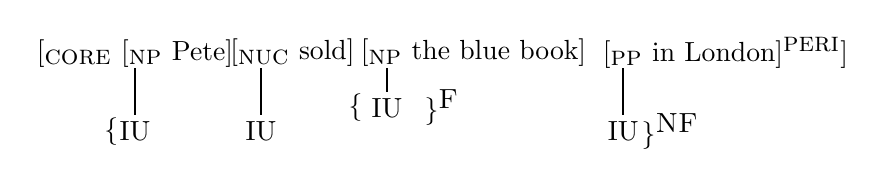
\begin{tikzpicture}[]
    \draw [xshift=0.0cm,yshift=0.99cm] node [] {[$_{\textsc{core}}$ [$_{\textsc{np}}$ Pete]}  ;
    \draw [xshift=2.0cm,yshift=1.0cm] node [] {[$_{\textsc{nuc}}$ sold]}  ;
    \draw [xshift=4.3cm,yshift=1.0cm] node [] {[$_{\textsc{np}}$ the blue book]}  ;
    \draw [xshift=7.5cm,yshift=1.0cm] node [] {[$_{\textsc{pp}}$ in London]$^{\textsc{peri}}$]}  ;
    %%
    \draw [line width=0.2mm] (0.0,0.8) -- (0.0,0.2) ;
    \draw [line width=0.2mm] (1.6,0.8) -- (1.6,0.2) ;
    \draw [line width=0.2mm] (3.2,0.8) -- (3.2,0.5) ;
    \draw [line width=0.2mm] (6.2,0.8) -- (6.2,0.2) ;
    %%
    \draw [xshift=0.0cm,yshift=0.0cm] node [] {IU}  ;
    \draw [xshift=1.6cm,yshift=0.0cm] node [] {IU}  ;
    \draw [xshift=3.2cm,yshift=0.3cm] node [] {IU}  ;
    \draw [xshift=6.2cm,yshift=0.0cm] node [] {IU}  ;
    %%
    \draw [xshift=-0.3cm,yshift=0.0cm] node [] {\{} ;
    \draw [xshift=6.8cm,yshift=0.0cm] node [] {\}$^{\textsc{NF}}$} ;
    \draw [xshift=2.8cm,yshift=0.3cm] node [] {\{} ;
    \draw [xshift=3.9cm,yshift=0.3cm] node [] {\}$^{\textsc{F}}$} ;
    \end{tikzpicture}\\
    %%%%%%%
    {\small{content of {\textsc{non-focus}}:\footnote{For a simplification in the representations, at some places we use the following abbreviations: \\
\avm{ $x$[\type*{person} name & pete ] } $\rightarrow$ \avm{ $x$[\type*{pete} ] },
\avm{ $y$[\type*{book} color & blue ] } $\rightarrow$ \avm{ $y$[\type*{blue book} ] },
\avm{ $z$[\type*{settlement} name & london ] } $\rightarrow$ \avm{ $z$[\type*{london} ] } 
}\hspace*{0.3cm}content of {\textsc{focus}}:\hspace*{0.5cm}\isi{pragmatic assertion}:}}\\[1mm]
    \begin{minipage}{3.6cm}
    {\scalebox{0.85}{
    \avm{$e$[\type*{selling} actor & $x$[\type*{pete}] \\ undg & $\boxed{2}$ \\ loc & $z$[\type*{london}]] }
    }}
    \end{minipage}
    %
    \begin{minipage}{3.1cm}
    {\scalebox{0.85}{
        \avm{ $y$[\type*{book}
                color & blue
            ] }
    }}
    \vspace*{0.95cm}
    \end{minipage}
    %
    \begin{minipage}{2cm}
    $\boxed{2} = y$ 
    \vspace*{1.0cm}
    \end{minipage}

\newpage
%%%%%%%%%%%%%%%%%%%%%%%%%%

    \ex\label{ex:loc.foc:Balogh}
    narrow adjunct \isi{focus}:\\[1mm]
    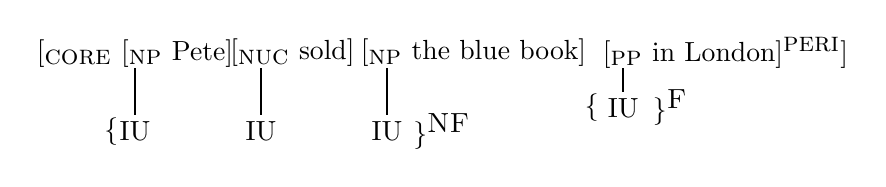
\begin{tikzpicture}[]
    \draw [xshift=0.0cm,yshift=0.99cm] node [] {[$_{\textsc{core}}$ [$_{\textsc{np}}$ Pete]}  ;
    \draw [xshift=2.0cm,yshift=1.0cm] node [] {[$_{\textsc{nuc}}$ sold]}  ;
    \draw [xshift=4.3cm,yshift=1.0cm] node [] {[$_{\textsc{np}}$ the blue book]}  ;
    \draw [xshift=7.5cm,yshift=1.0cm] node [] {[$_{\textsc{pp}}$ in London]$^{\textsc{peri}}$]}  ;
    %%%
    \draw [line width=0.2mm] (0.0,0.8) -- (0.0,0.2) ;
    \draw [line width=0.2mm] (1.6,0.8) -- (1.6,0.2) ;
    \draw [line width=0.2mm] (3.2,0.8) -- (3.2,0.2) ;
    \draw [line width=0.2mm] (6.2,0.8) -- (6.2,0.5) ;
    %%%
    \draw [xshift=0.0cm,yshift=0.0cm] node [] {IU}  ;
    \draw [xshift=1.6cm,yshift=0.0cm] node [] {IU}  ;
    \draw [xshift=3.2cm,yshift=0.0cm] node [] {IU}  ;
    \draw [xshift=6.2cm,yshift=0.3cm] node [] {IU}  ;
    %%%
    \draw [xshift=-0.3cm,yshift=0.0cm] node [] {\{} ;
    \draw [xshift=3.9cm,yshift=0.0cm] node [] {\}$^{\textsc{NF}}$} ;
    \draw [xshift=5.8cm,yshift=0.3cm] node [] {\{} ;
    \draw [xshift=6.8cm,yshift=0.3cm] node [] {\}$^{\textsc{F}}$} ;
    \end{tikzpicture}
    %%%%%%%
    {\small{content of {\textsc{non-focus}}:\hspace*{0.5cm}content of {\textsc{focus}}:\hspace*{0.5cm}\isi{pragmatic assertion}:}}\\[1mm]
    \begin{minipage}{3.6cm}
    {\scalebox{0.85}{
    \avm{$e$[\type*{selling} actor & $x$[\type*{pete}] \\ undg & $y$[\type*{blue book}] \\ loc & $\boxed{3}$] }
    }}
    \end{minipage}
    %
    \begin{minipage}{3.1cm}
    {\scalebox{0.85}{
        \avm{ $z$[\type*{settlement}
                name & london
            ] }
    }}
    \vspace*{0.95cm}
    \end{minipage}
    %
    \begin{minipage}{2cm}
    $\boxed{3} = z$ 
    \vspace*{1.0cm}
    \end{minipage}
     % end protectedex here
    \z
\z
%}

In \isi{complement focus} structures, the calculation of the content of the {\textsc{focus}} is straightforward: it equals the single \isi{IU} it contains. The content of the {\textsc{non-focus}} is calculated by a composition of its IUs, restricted by the syntactic composition, which is registered in the derivation tree. In other words, the unification of the IUs in the {\textsc{non-focus}} is constrained by the syntactic operations and the corresponding unifications of the values of the respective index features. 

The constructions where two (or more) complements are part of the {\textsc{focus}} are subsumed under the \isi{focus} structure type of \textit{multiple focus}, illustrated in (\ref{ex:mult.foc:Balogh}). Note that in case the \isi{IU} of the verb and the \isi{IU} of a complement (or the IUs of more complements) are within the {\textsc{focus}}, they do not form a multiple \isi{focus}, but are understood as a \isi{broad focus} structure. See, for example, the English example in (\ref{ex:no.mult.foc:Balogh}): a focal accent on the verb and on the indirect \isi{object} can only be interpreted with a (non-constituent) \isi{broad focus} structure. 

\ea\label{ex:no.mult.foc:Balogh}
Pete GAVE the blue book to SAM. \\
\isi{QUD}: \textit{What did Pete do with the blue book?}
\z

This suggests that we can only request the  specification of the value of an argument/adjunct if  the type of the event is known/given. In multiple \isi{focus} structures, the values of two (or possibly more) attributes need to be specified, which is provided by the IUs within the {\textsc{focus}}. This process, and thus the \isi{pragmatic assertion}, is parallel to the cases in \isi{complement focus} structures. 

%\newpage
\protectedex{
\ea\label{ex:mult.foc:Balogh}
    multiple \isi{focus} structure:\\[1mm]
    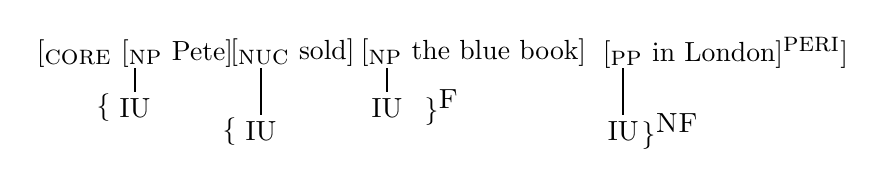
\begin{tikzpicture}[]
    \draw [xshift=0.0cm,yshift=0.99cm] node [] {[$_{\textsc{core}}$ [$_{\textsc{np}}$ Pete]}  ;
    \draw [xshift=2.0cm,yshift=1.0cm] node [] {[$_{\textsc{nuc}}$ sold]}  ;
    \draw [xshift=4.3cm,yshift=1.0cm] node [] {[$_{\textsc{np}}$ the blue book]}  ;
    \draw [xshift=7.5cm,yshift=1.0cm] node [] {[$_{\textsc{pp}}$ in London]$^{\textsc{peri}}$]}  ;
    %%%
    \draw [line width=0.2mm] (0.0,0.8) -- (0.0,0.5) ;
    \draw [line width=0.2mm] (1.6,0.8) -- (1.6,0.2) ;
    \draw [line width=0.2mm] (3.2,0.8) -- (3.2,0.5) ;
    \draw [line width=0.2mm] (6.2,0.8) -- (6.2,0.2) ;
    %%%
    \draw [xshift=0.0cm,yshift=0.3cm] node [] {IU}  ;
    \draw [xshift=1.6cm,yshift=0.0cm] node [] {IU}  ;
    \draw [xshift=3.2cm,yshift=0.3cm] node [] {IU}  ;
    \draw [xshift=6.2cm,yshift=0.0cm] node [] {IU}  ;
    %%%
    \draw [xshift=-0.4cm,yshift=0.3cm] node [] {\{} ;
    \draw [xshift=3.9cm,yshift=0.3cm] node [] {\}$^{\textsc{F}}$} ;
    \draw [xshift=1.2cm,yshift=0.0cm] node [] {\{} ;
    \draw [xshift=6.8cm,yshift=0.0cm] node [] {\}$^{\textsc{NF}}$} ;
    \end{tikzpicture}\\
    %%%%%%%
    {\small{content of {\textsc{non-focus}}:\hspace*{0.5cm}content of {\textsc{focus}}:\hspace*{0.5cm}\isi{pragmatic assertion}:}}\\[1mm]
    \begin{minipage}{3.6cm}
    {\scalebox{0.85}{
    \avm{$e$[\type*{selling} 
        actor & $\boxed{1}$ \\ 
        undg & $\boxed{2}$ \\ 
        loc & $z$[\type*{london}]
        ] }
    }}
    \end{minipage}
    %
    \begin{minipage}{3.1cm}
    {\scalebox{0.85}{
        \avm{ $x$[\type*{person}
                name & pete
            ] }
    }}\\[1mm]
    {\scalebox{0.85}{
        \avm{ $y$[\type*{book}
                color & blue
            ] }
    }}
    \vspace*{0.0cm}
    \end{minipage}
    %
    \begin{minipage}{2cm}
    $\boxed{1} = x$ \\[1mm]
    $\boxed{2} = y$ \\
    \vspace*{0.2cm}
    \end{minipage}
\z
}


\subsection{Verb focus and broad focus }\label{sec:broad.foc:Balogh}

The \isi{focus} structures in the previous section all reflected the resolving of an underlying issue where one (or more) of the complements are queried, i.e., the type of the eventuality is known/given (part of the {\textsc{non-focus}}), while the value of one (or more) of the attributes in the event description must be specified. Cases of verb \isi{focus} and \isi{broad focus} structures differ as here the type of the eventuality needs to be specified by the focal part, while some of the attributes can be (and often are) given. Therefore, the \isi{pragmatic assertion} is the type specification of the described eventuality, which can be simple as `type: selling' or complex as `type: selling the blue book'. To formally capture such complex types, the content of the {\textsc{focus}} can be seen as a \textit{frame type} \citep[introduced by][]{balogh:osswald:20}. The exact formal specification of such frame types and their relation to the content of the {\textsc{focus}} needs a more thorough investigation, which we leave for further work. Nevertheless, the example in (\ref{ex:v.foc:Balogh}) reflects this idea, although presenting the \isi{pragmatic assertion} still in an informal way. 

\ea\label{ex:v.foc:Balogh}
    verb \isi{focus}: \\
    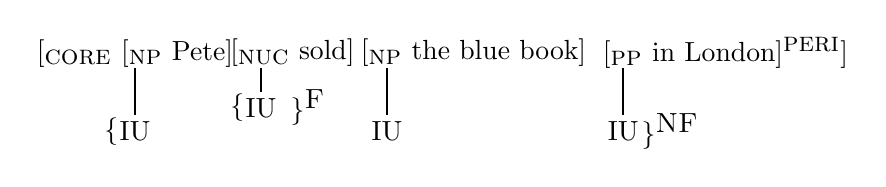
\begin{tikzpicture}[]
    \draw [xshift=0.0cm,yshift=0.99cm] node [] {[$_{\textsc{core}}$ [$_{\textsc{np}}$ Pete]}  ;
    \draw [xshift=2.0cm,yshift=1.0cm] node [] {[$_{\textsc{nuc}}$ sold]}  ;
    \draw [xshift=4.3cm,yshift=1.0cm] node [] {[$_{\textsc{np}}$ the blue book]}  ;
    \draw [xshift=7.5cm,yshift=1.0cm] node [] {[$_{\textsc{pp}}$ in London]$^{\textsc{peri}}$]}  ;
    %%
    \draw [line width=0.2mm] (0.0,0.8) -- (0.0,0.2) ;
    \draw [line width=0.2mm] (1.6,0.8) -- (1.6,0.5) ;
    \draw [line width=0.2mm] (3.2,0.8) -- (3.2,0.2) ;
    \draw [line width=0.2mm] (6.2,0.8) -- (6.2,0.2) ;
    %%
    \draw [xshift=0.0cm,yshift=0.0cm] node [] {IU}  ;
    \draw [xshift=1.6cm,yshift=0.3cm] node [] {IU}  ;
    \draw [xshift=3.2cm,yshift=0.0cm] node [] {IU}  ;
    \draw [xshift=6.2cm,yshift=0.0cm] node [] {IU}  ;
    %%
    \draw [xshift=-0.3cm,yshift=0.0cm] node [] {\{} ;
    \draw [xshift=6.8cm,yshift=0.0cm] node [] {\}$^{\textsc{NF}}$} ;
    \draw [xshift=1.3cm,yshift=0.3cm] node [] {\{} ;
    \draw [xshift=2.2cm,yshift=0.3cm] node [] {\}$^{\textsc{F}}$} ;
    \end{tikzpicture}\\
    %%%%%%%%%%
    {\small{content of {\textsc{non-focus}}:\hspace*{0.8cm}content of {\textsc{focus}}:\hspace*{0.5cm}\isi{pragmatic assertion}:}}\\[1mm]
    \begin{minipage}{4.0cm}
    {\scalebox{0.85}{
    \avm{$e$[\type*{event} 
        actor & $x$[\type*{pete}] \\
        undg & $y$[\type*{blue book}] \\
        loc & $z$[\type*{london}]
        ] }
    }}
    \end{minipage}
    %
    \begin{minipage}{3.1cm}
    {\scalebox{0.85}{
        \avm{$e$[\type*{selling} 
        actor & $x$ \\
        undg & $y$ 
        ] }
    }}
    \vspace*{0.5cm}
    \end{minipage}
    %
    \begin{minipage}{2cm}
    type of $e$ is `selling'
    \vspace*{0.9cm}
    \end{minipage}
\z

As illustrated in (\ref{ex:v.foc:Balogh}), in verb \isi{focus} structure, the {\textsc{focus}} contains the single \isi{IU} by the verb/main predicate. The {\textsc{non-focus}} contains the information that the given participants are functionally related under an eventuality of an unknown type.\footnote{The type specification `event' in the frame is highly underspecified.} This information is jointly derived on the basis of the derivation tree and the set of IUs. The IUs are all connected under the node $\alpha$, representing a yet unspecified eventuality. The {\textsc{focus}} provides the type specification: $e$ is of type `selling'. The {\scshape{actor}} and {\scshape{undergoer}} attributes represent the obligatory attributes and thus a restriction as a consequence of having the event type `selling'. 

When the {\textsc{focus}} contains the IUs of the verb and one (or more) of its arguments/adjuncts, we talk about a \isi{broad focus} structure. Although these cases can be divided into further subtypes, their \isi{pragmatic assertion} is uniformly captured as providing a possibly complex event type (in terms of frame types). The special subtypes that can be distinguished are: (i) cases where the {\textsc{non-focus}} is a singleton set (\ref{ex:broad.foc:Balogh}), this type including the traditional ``predicate \isi{focus}'' structure; (ii) cases where both the {\textsc{non-focus}} and the {\textsc{focus}} are non-empty, non-singleton sets (\ref{ex:nonconst.foc:Balogh}), these cases being often referred to as ``non-constituent'' \isi{focus} in other approaches, and (iii) cases where the {\textsc{non-focus}} is an empty set, which is referred to as ``sentence \isi{focus}''. In the latter \isi{focus} structure, all IUs within the sentence are in the {\textsc{focus}}, while the {\textsc{non-focus}} is empty. In such cases, the content of the whole sentence is considered new information. Nevertheless, an empty {\textsc{non-focus}} does not mean that such sentences are unrelated to the local discourse context (see, for example, the notion of ``stage topic'' by \citealt{es:07}). 

\ea\label{ex:broad.foc:Balogh}
    \ea\label{ex:pred.foc:Balogh}
    (traditional) predicate \isi{focus}:\\[1mm]
    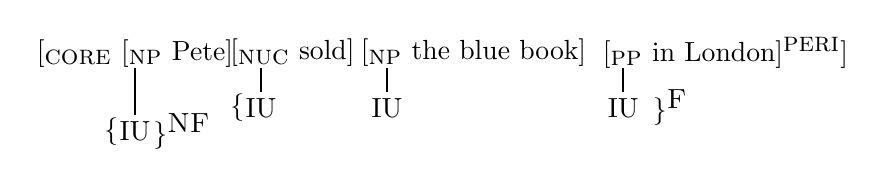
\begin{tikzpicture}[]
    \draw [xshift=0.0cm,yshift=0.99cm] node [] {[$_{\textsc{core}}$ [$_{\textsc{np}}$ Pete]}  ;
    \draw [xshift=2.0cm,yshift=1.0cm] node [] {[$_{\textsc{nuc}}$ sold]}  ;
    \draw [xshift=4.3cm,yshift=1.0cm] node [] {[$_{\textsc{np}}$ the blue book]}  ;
    \draw [xshift=7.5cm,yshift=1.0cm] node [] {[$_{\textsc{pp}}$ in London]$^{\textsc{peri}}$]}  ;
    %%
    \draw [line width=0.2mm] (0.0,0.8) -- (0.0,0.2) ;
    \draw [line width=0.2mm] (1.6,0.8) -- (1.6,0.5) ;
    \draw [line width=0.2mm] (3.2,0.8) -- (3.2,0.5) ;
    \draw [line width=0.2mm] (6.2,0.8) -- (6.2,0.5) ;
    %%
    \draw [xshift=0.0cm,yshift=0.0cm] node [] {IU}  ;
    \draw [xshift=1.6cm,yshift=0.3cm] node [] {IU}  ;
    \draw [xshift=3.2cm,yshift=0.3cm] node [] {IU}  ;
    \draw [xshift=6.2cm,yshift=0.3cm] node [] {IU}  ;
    %%
    \draw [xshift=-0.3cm,yshift=0.0cm] node [] {\{} ;
    \draw [xshift=0.6cm,yshift=0.0cm] node [] {\}$^{\textsc{NF}}$} ;
    \draw [xshift=1.3cm,yshift=0.3cm] node [] {\{} ;
    \draw [xshift=6.8cm,yshift=0.3cm] node [] {\}$^{\textsc{F}}$} ;
    \end{tikzpicture}\\
    %%%%%%%%%%
    {\small{content of {\textsc{non-focus}}:\hspace*{0.4cm}content of {\textsc{focus}}:\hspace*{1.0cm}\isi{pragmatic assertion}:}}\\[1mm]
    \begin{minipage}{3.5cm}
    {\scalebox{0.85}{
    \avm{$e$[\type*{event} 
        actor & $x$[\type*{pete}] 
        ] }
    }}
    \vspace*{0.9cm}
    \end{minipage}
    %
    \begin{minipage}{3.6cm}
    {\scalebox{0.85}{
        \avm{$e$[\type*{selling} 
        actor & $x$ \\
        undg & $y$[\type*{blue book}]  \\
        loc & $z$[\type*{london}]  \\
        ] }
    }}
    \end{minipage}
    %
    \begin{minipage}{2cm}
    type of $e$ is `selling the blue book in London'
    \end{minipage}

%\newpage
%%%%%%%%%%%%%%%%%%%%%%%%%%%%%%%%%%%%%%%%%%%%%
\protectedex{
    \ex\label{ex:obj.top.foc:Balogh}
    relationally given {\scshape{undergoer}}:\\[1mm]
    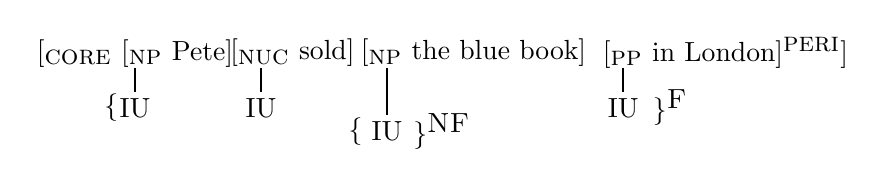
\begin{tikzpicture}[]
    \draw [xshift=0.0cm,yshift=0.99cm] node [] {[$_{\textsc{core}}$ [$_{\textsc{np}}$ Pete]}  ;
    \draw [xshift=2.0cm,yshift=1.0cm] node [] {[$_{\textsc{nuc}}$ sold]}  ;
    \draw [xshift=4.3cm,yshift=1.0cm] node [] {[$_{\textsc{np}}$ the blue book]}  ;
    \draw [xshift=7.5cm,yshift=1.0cm] node [] {[$_{\textsc{pp}}$ in London]$^{\textsc{peri}}$]}  ;
    %%
    \draw [line width=0.2mm] (0.0,0.8) -- (0.0,0.5) ;
    \draw [line width=0.2mm] (1.6,0.8) -- (1.6,0.5) ;
    \draw [line width=0.2mm] (3.2,0.8) -- (3.2,0.2) ;
    \draw [line width=0.2mm] (6.2,0.8) -- (6.2,0.5) ;
    %%
    \draw [xshift=0.0cm,yshift=0.3cm] node [] {IU}  ;
    \draw [xshift=1.6cm,yshift=0.3cm] node [] {IU}  ;
    \draw [xshift=3.2cm,yshift=0.0cm] node [] {IU}  ;
    \draw [xshift=6.2cm,yshift=0.3cm] node [] {IU}  ;
    %%
    \draw [xshift=-0.3cm,yshift=0.3cm] node [] {\{} ;
    \draw [xshift=6.8cm,yshift=0.3cm] node [] {\}$^{\textsc{F}}$} ;
    \draw [xshift=2.8cm,yshift=0.0cm] node [] {\{} ;
    \draw [xshift=3.9cm,yshift=0.0cm] node [] {\}$^{\textsc{NF}}$} ;
    \end{tikzpicture}\\
    %%%%%%%%%%
    {\small{content of {\textsc{non-focus}}:\hspace*{0.4cm}content of {\textsc{focus}}:\hspace*{0.9cm}\isi{pragmatic assertion}:}}\\[1mm]
    \begin{minipage}{3.6cm}
    {\scalebox{0.85}{
    \avm{$e$[\type*{event} 
        undg & $y$[\type*{blue book}] 
        ] }
    }}
    \vspace*{0.9cm}
    \end{minipage}
    %
    \begin{minipage}{3.4cm}
    {\scalebox{0.85}{
        \avm{$e$[\type*{selling} 
        actor & $x$[\type*{pete}] \\
        undg & $y$  \\
        loc & $z$[\type*{london}]  \\
        ] }
    }}
    \end{minipage}
    %
    \begin{minipage}{2cm}
    type of $e$ is `selling by Pete in London'
    \end{minipage}
    } % end protectedex here
    \z    
\z


In both examples in (\ref{ex:broad.foc:Balogh}), the {\textsc{non-focus}} expresses a yet unspecified eventuality, of which one of the participants is specified. These structures correspond to the topic-comment division, however, we claim that the topic-comment structure represents a different aspect of \isi{IS}, that needs to be represented separately. It also requires a representation of the referential structure of the sentence in context, that is not yet included in our model. 

The examples in (\ref{ex:nonconst.foc:Balogh}) illustrate different cases where the verb together with an argument or adjunct form the {\textsc{focus}}. In our approach, these cases are captured parallel to the ones in (\ref{ex:v.foc:Balogh}) and (\ref{ex:broad.foc:Balogh}): the uniform core function of focusing is the specification of the (possibly complex) type of the eventuality under discussion. 

\ea\label{ex:nonconst.foc:Balogh}
    \ea\label{ex:subj.v.foc:Balogh}
\begin{nobreak}
    focal \isi{subject} + V:\\[1mm]
    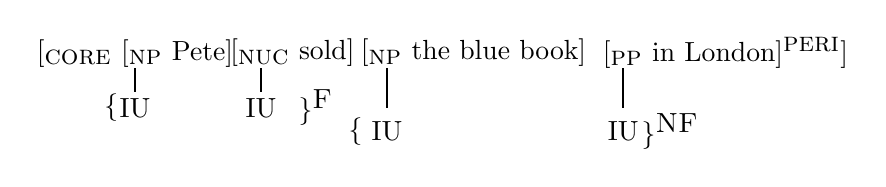
\begin{tikzpicture}[]
    \draw [xshift=0.0cm,yshift=0.99cm] node [] {[$_{\textsc{core}}$ [$_{\textsc{np}}$ Pete]}  ;
    \draw [xshift=2.0cm,yshift=1.0cm] node [] {[$_{\textsc{nuc}}$ sold]}  ;
    \draw [xshift=4.3cm,yshift=1.0cm] node [] {[$_{\textsc{np}}$ the blue book]}  ;
    \draw [xshift=7.5cm,yshift=1.0cm] node [] {[$_{\textsc{pp}}$ in London]$^{\textsc{peri}}$]}  ;
    %%
    \draw [line width=0.2mm] (0.0,0.8) -- (0.0,0.5) ;
    \draw [line width=0.2mm] (1.6,0.8) -- (1.6,0.5) ;
    \draw [line width=0.2mm] (3.2,0.8) -- (3.2,0.3) ;
    \draw [line width=0.2mm] (6.2,0.8) -- (6.2,0.3) ;
    %%
    \draw [xshift=0.0cm,yshift=0.3cm] node [] {IU}  ;
    \draw [xshift=1.6cm,yshift=0.3cm] node [] {IU}  ;
    \draw [xshift=3.2cm,yshift=0.0cm] node [] {IU}  ;
    \draw [xshift=6.2cm,yshift=0.0cm] node [] {IU}  ;
    %%
    \draw [xshift=-0.3cm,yshift=0.3cm] node [] {\{} ;
    \draw [xshift=2.3cm,yshift=0.3cm] node [] {\}$^{\textsc{F}}$} ;
    \draw [xshift=2.8cm,yshift=0.0cm] node [] {\{} ;
    \draw [xshift=6.8cm,yshift=0.0cm] node [] {\}$^{\textsc{NF}}$} ;
    \end{tikzpicture}\\
    %%%%%%%%%%
    {\small{content of {\textsc{non-focus}}:\hspace*{0.5cm}content of {\textsc{focus}}:\hspace*{0.7cm}\isi{pragmatic assertion}:}}\\[1mm]
    \begin{minipage}{3.5cm}
    {\scalebox{0.85}{
    \avm{$e$[\type*{event} 
        undg & $y$[\type*{blue book}] \\
        loc & $z$[\type*{london}]
        ] }
    }}
    \end{minipage}
    %
    \begin{minipage}{3.4cm}
    {\scalebox{0.85}{
        \avm{$e$[\type*{selling} 
        actor & $x$[\type*{pete}] \\
        undg & $y$ 
        ] }
    }}
    \end{minipage}
    %
    \begin{minipage}{2.0cm}
    type of $e$ is `selling by Pete'
    \end{minipage}
\end{nobreak}

\medskip
%%%%%%%%%%%%%%%%%%%%%%%%%%%%%%%%%%%
    \ex\label{ex:v.loc.foc:Balogh}
    focal V + adjunct:\\[1mm]
    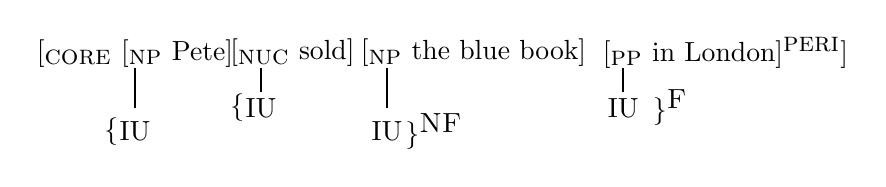
\begin{tikzpicture}[]
    \draw [xshift=0.0cm,yshift=0.99cm] node [] {[$_{\textsc{core}}$ [$_{\textsc{np}}$ Pete]}  ;
    \draw [xshift=2.0cm,yshift=1.0cm] node [] {[$_{\textsc{nuc}}$ sold]}  ;
    \draw [xshift=4.3cm,yshift=1.0cm] node [] {[$_{\textsc{np}}$ the blue book]}  ;
    \draw [xshift=7.5cm,yshift=1.0cm] node [] {[$_{\textsc{pp}}$ in London]$^{\textsc{peri}}$]}  ;
    %%
    \draw [line width=0.2mm] (0.0,0.8) -- (0.0,0.3) ;
    \draw [line width=0.2mm] (1.6,0.8) -- (1.6,0.5) ;
    \draw [line width=0.2mm] (3.2,0.8) -- (3.2,0.3) ;
    \draw [line width=0.2mm] (6.2,0.8) -- (6.2,0.5) ;
    %%
    \draw [xshift=0.0cm,yshift=0.0cm] node [] {IU}  ;
    \draw [xshift=1.6cm,yshift=0.3cm] node [] {IU}  ;
    \draw [xshift=3.2cm,yshift=0.0cm] node [] {IU}  ;
    \draw [xshift=6.2cm,yshift=0.3cm] node [] {IU}  ;
    %%
    \draw [xshift=1.3cm,yshift=0.3cm] node [] {\{} ;
    \draw [xshift=6.8cm,yshift=0.3cm] node [] {\}$^{\textsc{F}}$} ;
    \draw [xshift=-0.3cm,yshift=0.0cm] node [] {\{} ;
    \draw [xshift=3.8cm,yshift=0.0cm] node [] {\}$^{\textsc{NF}}$} ;
    \end{tikzpicture}\\
    %%%%%%%%%%
    {\small{content of {\textsc{non-focus}}:\hspace*{0.5cm}content of {\textsc{focus}}:\hspace*{0.7cm}\isi{pragmatic assertion}:}}\\[1mm]
    \begin{minipage}{3.5cm}
    {\scalebox{0.85}{
    \avm{$e$[\type*{event} 
        actor & $x$[\type*{pete}] \\
        undg & $y$[\type*{blue book}]
        ] }
    }}
    \end{minipage}
    %
    \begin{minipage}{3.4cm}
    {\scalebox{0.85}{
        \avm{$e$[\type*{selling} 
        actor & $x$ \\
        undg & $y$ \\
        loc & $z$[\type*{london}]
        ] }
    }}
    \end{minipage}
    %
    \begin{minipage}{2cm}
    type of $e$ is `selling in London'
    \end{minipage}
    \z
\z


\section{Conclusion and further issues }\label{sec:concl:Balogh}

\subsection{Concluding remarks}
In this paper, we introduced a first proposal towards a grammar formalism that offers a novel approach to the representation and analysis of \isi{information structure}, in particular the \isi{focus} structure of the sentence. Our proposal is based on the theoretical grounds of \isi{Role and Reference Grammar} \citep{vvlp:97,vanvalin:05} and \citeauthor{lambrecht:94}'s (\citeyear{lambrecht:94}) theory of \isi{information structure}, formally implemented using \isi{Tree-Wrapping Grammar} \citep{kallm:etal:13,kallm:ossw:23} and decompositional \isi{frame semantics} \citep{kallm:ossw:13,lobner:14,petersen:15}.

The core motivating phenomenon in this paper is ``non-constituent \isi{focus}'', that is problematic for traditional compositional analyses capturing \isi{focus} structure with the use of syntactic F-marking. The particular problems with this special \isi{information structure} are addressed by \citet{buring:16}, who offers a solution without F-marking, using Unalternative Semantics \citep{buring:06,buring:15}. B\"uring's approach offers a highly appropriate and elegant solution for semantic theories where \isi{focus} is defined as the source of alternatives. However, this approach not only eliminates the syntactic F-marking, but also the representation of the \isi{focus} structure. We argue that from a linguistic and grammatical perspective this can be disadvantageous, since \isi{focus} structure plays an essential role in the different stages at the linking between syntax and semantics \citep[][]{bentley:23,lvv:23,vanvalin:05}.

In our approach, we aim to uniformly capture the various \isi{focus} structures, in a way that straightforwardly extends to cases previously referred to as ``non-constituent \isi{focus}''. The core of our proposal is that \isi{focus} structure is not directly determined on the nodes of the constituent structure. Instead, \isi{information structure} (containing \isi{focus} structure) is represented in a separate module, which is linked both to syntax and to semantics. Consequently, the structures found at the level of \isi{IS} do not need to be parallel to the structures found at the level of syntax, which is essentially correct, and naturally prevents the issues raised by ``non-constituent'' \isi{focus} in traditional compositional accounts. The general architecture of \isi{RRG} and our representation of \isi{IS} are considerably different. In our approach, information units (IUs) play an essential role in determining the \isi{focus} structure. Crucially, the IUs are linked to syntactic domains, but the \isi{focus} structure is not read off the syntactic structure. Therefore, when the basic IUs are defined, any combination of them can make up the content of the {\textsc{focus}}. The IUs are determined structurally together with the corresponding pieces of semantic representations. Focus structure is essentially represented as a partition of the set of IUs into two IS-domains: the {\textsc{non-focus}} and the {\textsc{focus}}. The core function of focusing is a \isi{pragmatic structuring}, represented by the content of the {\textsc{non-focus}} and the {\textsc{focus}} (which correspond to the underlying issue and the \isi{focus} respectively), and the \isi{pragmatic assertion}, which is seen as a special relation between the issue and the content of {\textsc{focus}}. The formal derivation of the \isi{focus} structure and the content of the IS-domains is uniform across all cases. A difference in \isi{pragmatic assertion} is proposed based on whether the verb/main predicate is part of the {\textsc{focus}}. 


\subsection{Further issues}
As any new proposal, our approach has several loose ends, that ask for further investigation in terms of formalization and empirical coverage. 
For the formalization, we have two main tasks directly ahead of us: (i) the formal derivation/calculation of the content of the {\textsc{non-focus}} and the {\textsc{focus}} needs to be worked out in more detail, and (ii) the representation of their relation, i.e., the \isi{pragmatic assertion}, needs to be formally characterized. As for the first issue, we proposed in this paper that this calculation is determined by the IUs and the derivation tree. Currently, we have two basic processes: in argument \isi{focus} structures, the sub-tree corresponding to the \isi{IU} within the {\textsc{focus}} is cut-off the derivation tree, while the remaining tree determines the content of the {\textsc{non-focus}}; in \isi{broad focus} structures, the derivation tree is divided into two sub-trees, both including a copy of the root node (which reflects that the content of the two domains describes information on the same eventuality). This needs to be refined in a more uniform way that applies to further problematic cases as well. We are currently exploring the idea of defining a more flexible composition, where we model the background-\isi{focus} distinction within a construction, such that certain pragmatic factors are reflected in syntactic composition. This revision would also be seen as part of the formal characterization of the linking between syntax and pragmatics, which is core to our modular grammar architecture. Working out the second issue, our initial proposal is to include complex frame types. The formal definitions of this idea are currently being developed. 

In this paper, we discussed rather basic constructions, that best served as a starting point of our formal grammatical model, and best facilitate the aim of introducing our approach and the basic processes globally. Needless to say, for a comprehensive model, we need to verify that our approach is applicable to more phenomena and complex constructions cross-linguistically. Currently, we are investigating different types of adjunct \isi{modifiers} that do not necessarily introduce an attribute in the event description (e.g., {\emph{almost}}, {\emph{completely}}, {\emph{intentionally}}), clausal adjuncts and complex noun phrases. The core issues are what exactly counts as a basic \isi{IU} and how to capture IUs and IS-domains in embedded constructions. Furthermore, we need to extend our proposal to further languages beyond English. Currently, we are looking at different case studies in Hungarian, Japanese and Lakota. 

\subsection{A brief note on related formalisms}

While our approach is based on the theoretical grounds of \isi{RRG}, the core proposal of the formal representation of the \isi{focus} structure does not strictly require RRG-like syntactic structures. From the theoretical point of view, the important aspect of the grammatical model is its modular architecture without the primacy of syntax, and the linking between the different representation levels. The linguistic theory of \isi{RRG} is developed proposing such an architecure, therefore it provides an excellent ground for our formal implementation. Nevertheless, the core proposal in this paper can be worked out with a standard Lexicalized Tree-Adjoining Grammar (LTAG) with frame-based semantics, and possibly also within a construction-based Lexical Functional Grammar (LFG) model \citep[e.g.,][]{findlay:23}. The theories of \isi{RRG} and LFG both argue for a modular grammar architecture, which raises the issue whether the two offer similar or comparable approaches to \isi{information structure}. The possibilities of the above mentioned alternative formal models, as well as a thorough comparison of the approaches to \isi{information structure} within \isi{RRG} \citep[see, e.g.,][]{vvlp:97,vanvalin:05,bentley:23} and within LFG \citep[see, e.g.,][]{butt:king:96,dalrymple:nikolaeva:11,dalrymple:etal:19,zaenen:23} are left for further work. 

\section*{Acknowledgements}
The research reported in this paper is supported by the Deutsche Forschungsgemeinschaft (DFG, grant number BA 7299/2-1). 

\sloppy
\printbibliography[heading=subbibliography,notkeyword=this]

\end{document}
